% !TeX program = xelatex
\documentclass[12pt,a4paper]{report}

\usepackage[a4paper,left=3cm,right=2cm,top=2.5cm,bottom=2.5cm]{geometry}
\usepackage{fontspec}
\IfFontExistsTF{Times New Roman}{
  \setmainfont{Times New Roman}
  \setsansfont{Times New Roman}
}{
  \setmainfont{Liberation Serif}
  \setsansfont{Liberation Sans}
}
\usepackage{graphicx}
\usepackage{array}
\usepackage{tabularx}
\usepackage{xltabular}
\usepackage{booktabs}
\usepackage{float}
\usepackage{caption}
\usepackage{enumitem}
\usepackage{indentfirst}
\usepackage{eso-pic}
\usepackage{setspace}
\usepackage{titlesec}
\usepackage{tocloft}
\usepackage{url}
\usepackage{hyperref}

% Thay các thông tin này trước khi biên dịch.
\newcommand{\UniversityName}{HỌC VIỆN CÔNG NGHỆ BƯU CHÍNH VIỄN THÔNG}
\newcommand{\FacultyName}{KHOA CÔNG NGHỆ THÔNG TIN 1}
\newcommand{\DepartmentName}{BỘ MÔN TIN HỌC CƠ SỞ}
\newcommand{\ReportTitle}{HỆ THỐNG QUẢN LÝ KÝ TÚC XÁ PTIT}
\newcommand{\AdvisorName}{ThS. Nguyễn Đình Hiến}
\newcommand{\StudentName}{}
\newcommand{\StudentID}{}
\newcommand{\ClassName}{}
\newcommand{\GroupNumber}{12}
\newcommand{\ReportPlace}{Hà Nội}
\newcommand{\ReportMonth}{11}
\newcommand{\ReportYear}{2026}

\hypersetup{
  colorlinks=true,
  linkcolor=black,
  pdftitle={\ReportTitle},
  pdfauthor={\StudentName}
}
\renewcommand{\contentsname}{MỤC LỤC}
\renewcommand{\listfigurename}{DANH MỤC HÌNH VẼ}
\renewcommand{\listtablename}{DANH MỤC BẢNG BIỂU}
\renewcommand{\figurename}{Hình}
\renewcommand{\tablename}{Bảng}
\renewcommand{\chaptername}{CHƯƠNG}
\renewcommand{\cftchappresnum}{Chương~}
\renewcommand{\cftchapaftersnum}{\quad}
\setlength{\cftchapnumwidth}{2.25cm}
\renewcommand{\cfttoctitlefont}{\hfill\bfseries\Large}
\renewcommand{\cftaftertoctitle}{\hfill}
\renewcommand{\cftloftitlefont}{\hfill\bfseries\Large}
\renewcommand{\cftafterloftitle}{\hfill}
\renewcommand{\cftlottitlefont}{\hfill\bfseries\Large}
\renewcommand{\cftafterlottitle}{\hfill}
\renewcommand{\cftchapfont}{\bfseries}
\renewcommand{\cftchappagefont}{\bfseries}
\setlength{\cftbeforechapskip}{6pt}
\setlength{\cftsecindent}{1.25em}
\setlength{\cftsubsecindent}{2.5em}
\renewcommand{\cfttabpresnum}{Bảng~}
\renewcommand{\cfttabaftersnum}{\quad}
\setlength{\cfttabnumwidth}{2.4cm}
\renewcommand{\cftfigpresnum}{Hình~}
\renewcommand{\cftfigaftersnum}{\quad}
\setlength{\cftfignumwidth}{2.4cm}
\setcounter{tocdepth}{2}
\titleformat{\chapter}[block]
  {\normalfont\bfseries\centering\Large}
  {\chaptername\ \thechapter.}
  {0.6em}
  {\Large\MakeUppercase}
\titlespacing*{\chapter}{0pt}{0pt}{1.2cm}
\titleformat{\section}{\normalfont\bfseries\large}{\thesection.}{0.6em}{}
\titleformat{\subsection}{\normalfont\bfseries\normalsize}{\thesubsection.}{0.6em}{}
\titleformat{\subsubsection}{\normalfont\bfseries\normalsize}{\thesubsubsection.}{0.6em}{}
\titleformat{\paragraph}[hang]{\normalfont\bfseries\normalsize}{}{0pt}{}
\titlespacing*{\paragraph}{0pt}{0.8em}{0.4em}
\setstretch{1.15}
\setlength{\parindent}{1.25cm}
\setlength{\parskip}{0.25em}
\renewcommand{\arraystretch}{1.12}
\captionsetup{font=small,labelfont=bf,skip=8pt}
\captionsetup[table]{position=top}
\captionsetup[figure]{position=bottom}
\setlist[itemize]{topsep=4pt,itemsep=2pt,parsep=0pt}
\setlist[enumerate]{topsep=4pt,itemsep=2pt,parsep=0pt}

\begin{document}

% Trang bìa được dựng theo mẫu tham khảo trong assets/image.png.
\begin{titlepage}
\thispagestyle{empty}
\AddToShipoutPictureBG*{%
  \AtPageLowerLeft{%
    \setlength{\unitlength}{1mm}%
    \put(12,12){\framebox(186,273){}}%
    \put(13,13){\framebox(184,271){}}%
  }%
}
\begin{center}
\vspace*{-0.8cm}
{\large\parbox{0.9\textwidth}{\centering \UniversityName}\par}
\vspace{0.1cm}
{\bfseries\large \FacultyName\par}
\vspace{0.05cm}
\rule[0.5ex]{2.5cm}{0.3pt}\,{\small o0o}\,\rule[0.5ex]{2.5cm}{0.3pt}

\vspace{0.7cm}
\IfFileExists{assets/ptit_logo.png}{%
  
\includegraphics[width=3.1cm]{assets/ptit_logo.png}%
}{\fbox{\parbox[c][3.1cm][c]{3.1cm}{\centering Logo PTIT}}}

\vspace{1.7cm}
{\bfseries\Large BÁO CÁO BÀI TẬP LỚN\par}
\vspace{0.35cm}
{\bfseries\large\parbox{0.88\textwidth}{\centering PHÂN TÍCH \& THIẾT KẾ HỆ THỐNG THÔNG TIN}\par}

\vspace{0.65cm}
{\bfseries\Large\parbox{0.88\textwidth}{\centering \ReportTitle}\par}

\vspace{1.2cm}
\renewcommand{\arraystretch}{1.05}
\begin{tabular}{>{\bfseries}p{5.0cm}p{0.35cm}p{6.3cm}}
Giảng viên hướng dẫn & : & \AdvisorName \\
Nhóm môn học & : & \GroupNumber \\
Nhóm bài tập lớn & : & 05 \\
\end{tabular}

\vspace{0.3cm}
{\bfseries Sinh viên thực hiện\par}
\vspace{0.1cm}
\begin{tabular}{|>{\centering\arraybackslash}p{6.5cm}|>{\centering\arraybackslash}p{4cm}|}
\hline
\bfseries Tên sinh viên & \bfseries Mã sinh viên \\
\hline
Đinh Việt Dũng & B23DCKH031 \\
\hline
Nguyễn Vĩnh Tùng & B23DCKH130 \\
\hline
Nguyễn Văn Tuấn & B23DCKH128 \\
\hline
Lê Xuân Nhân & B23DCKH083 \\
\hline
Đỗ Quang Huân & B23DCKH051 \\
\hline
\end{tabular}

\vfill
{\bfseries \ReportPlace{}, \ReportMonth/\ReportYear\par}
\vspace*{0.15cm}
\end{center}
\end{titlepage}

\clearpage
\setcounter{page}{2}
\pagestyle{plain}
\clearpage
\chapter*{LỜI MỞ ĐẦU}
\phantomsection
\addcontentsline{toc}{chapter}{LỜI MỞ ĐẦU}

Trong xu thế chuyển đổi số mạnh mẽ hiện nay, việc ứng dụng công nghệ thông tin vào công tác quản trị và hỗ trợ sinh viên tại các cơ sở giáo dục đại học đóng vai trò then chốt nhằm nâng cao hiệu quả vận hành và chất lượng dịch vụ. Tại Học viện Công nghệ Bưu chính Viễn thông, ký túc xá là đơn vị hỗ trợ thiết yếu, gắn liền trực tiếp với đời sống sinh hoạt của đông đảo sinh viên. Tuy nhiên, công tác quản lý lưu trú trên thực tế bao gồm nhiều nghiệp vụ phức tạp, liên kết chặt chẽ theo một vòng đời khép kín: từ quản lý phòng và giường, tiếp nhận đăng ký giữ chỗ, thiết lập hợp đồng, phát hành và thanh toán phí nội trú, cho đến hoàn tất thủ tục trả phòng. Việc quản lý bằng sổ sách truyền thống hay tệp bảng tính rời rạc dễ dẫn đến sai lệch trạng thái chỗ ở, trùng lặp hợp đồng và khó đối soát dữ liệu. Xuất phát từ yêu cầu thực tiễn đó, nhóm sinh viên lựa chọn đề tài \textbf{“Hệ thống quản lý ký túc xá PTIT”} cho bài tập lớn học phần Phân tích và thiết kế hệ thống thông tin.

Mục tiêu chính của đề tài là chuẩn hóa và mô hình hóa toàn diện quy trình quản lý vòng đời chỗ ở của sinh viên. Vận dụng phương pháp phân tích và thiết kế hướng đối tượng (OOAD) cùng ngôn ngữ mô hình hóa hợp nhất (UML), báo cáo tập trung xác định các tác nhân, phân tích yêu cầu chức năng, hệ thống hóa 12 quy tắc ràng buộc nghiệp vụ (Business Rules), xây dựng ma trận phân quyền, đặc tả chi tiết Use Case và thiết kế các biểu đồ hoạt động xuyên suốt. Đồng thời, nhóm đề xuất định hướng kiến trúc công nghệ hiện đại kết hợp ReactJS ở phía giao diện người dùng, Java xử lý dịch vụ backend, hệ quản trị cơ sở dữ liệu quan hệ PostgreSQL đảm bảo tính toàn vẹn và Redis hỗ trợ tra cứu nhanh cũng như kiểm soát giữ chỗ tạm thời.

Báo cáo bài tập lớn được kết cấu thành hai chương nội dung chính cùng các phần bổ trợ:
\begin{itemize}[nosep,leftmargin=1.5em]
\item \textbf{Chương 1: Giới thiệu đề tài và lựa chọn công nghệ} --- Trình bày lý do chọn đề tài, mục tiêu, kết quả dự kiến, phạm vi hệ thống, quy trình nghiệp vụ tổng quát và các công nghệ đề xuất.
\item \textbf{Chương 2: Phân tích hệ thống} --- Khảo sát hiện trạng, hệ thống hóa các quy tắc nghiệp vụ then chốt (BR01--BR12), xây dựng biểu đồ Use Case tổng quát, ma trận tác nhân -- Use Case và đặc tả chi tiết các Use Case chính.
\item \textbf{Kết luận và hướng phát triển} --- Tổng kết kết quả đạt được, chỉ ra những hạn chế và đề xuất các hướng mở rộng hệ thống trong tương lai.
\end{itemize}

Nhóm chúng em xin bày tỏ lòng biết ơn chân thành tới Ban giám hiệu Học viện Công nghệ Bưu chính Viễn thông, các thầy cô giáo Khoa Công nghệ Thông tin 1 và Bộ môn Tin học cơ sở đã tạo điều kiện học tập thuận lợi. Đặc biệt, nhóm xin gửi lời cảm ơn sâu sắc nhất tới thầy \textbf{ThS. Nguyễn Đình Hiến}, người đã tận tâm giảng dạy, định hướng đề tài và đóng góp những ý kiến quý báu giúp nhóm hoàn thành bài báo cáo này.

Do giới hạn về thời gian và kiến thức thực tế, bài báo cáo khó tránh khỏi những thiếu sót. Nhóm kính mong nhận được những góp ý, chỉ bảo của thầy cô và các bạn để đề tài ngày càng hoàn thiện hơn.

\clearpage
\phantomsection
\addcontentsline{toc}{chapter}{\contentsname}
\tableofcontents
\clearpage
\chapter*{DANH MỤC TỪ VIẾT TẮT}
\phantomsection
\addcontentsline{toc}{chapter}{DANH MỤC TỪ VIẾT TẮT}

\begin{center}
\begin{tabularx}{0.9\textwidth}{>{\bfseries}p{0.16\textwidth}X}
BR & Business Rule (quy tắc nghiệp vụ) \\
KTX & Ký túc xá \\
PTIT & Học viện Công nghệ Bưu chính Viễn thông \\
SV & Sinh viên \\
UC & Use Case (ca sử dụng) \\
UML & Unified Modeling Language (ngôn ngữ mô hình hóa thống nhất) \\
\end{tabularx}
\end{center}

\clearpage
\phantomsection
\addcontentsline{toc}{chapter}{\listtablename}
\listoftables
\clearpage
\phantomsection
\addcontentsline{toc}{chapter}{\listfigurename}
\listoffigures

\clearpage
\chapter{GIỚI THIỆU ĐỀ TÀI VÀ LỰA CHỌN CÔNG NGHỆ}

\section{Giới thiệu đề tài}

\subsection{Lý do chọn đề tài}

Ký túc xá là một bộ phận hỗ trợ trực tiếp đời sống học tập của sinh viên. Trong quá trình vận hành, cán bộ phải theo dõi số lượng phòng và giường, tiếp nhận nhu cầu ở nội trú, bố trí chỗ ở, lập hợp đồng, ghi nhận các khoản phí và xử lý việc trả phòng. Những nghiệp vụ này liên kết chặt chẽ với nhau vì một thay đổi ở trạng thái giường có thể ảnh hưởng đến kết quả tìm phòng, yêu cầu đặt phòng, hợp đồng và khả năng tiếp nhận sinh viên mới.

Khi dữ liệu được ghi chép ở nhiều sổ hoặc tệp riêng lẻ, cán bộ khó xác định trạng thái phòng tại cùng một thời điểm. Một giường có thể đã được giữ nhưng vẫn xuất hiện trong danh sách còn chỗ, hợp đồng đã kết thúc nhưng trạng thái giường chưa được cập nhật, khoản phí đã thanh toán nhưng thông tin chưa được phản ánh kịp thời. Các sai lệch này làm tăng thời gian đối chiếu và có thể dẫn đến bố trí trùng chỗ hoặc cung cấp thông tin không chính xác cho sinh viên.

Sinh viên cũng cần một kênh thống nhất để tìm phòng phù hợp, gửi yêu cầu đặt phòng, theo dõi khoản phí và đề nghị trả phòng. Nếu mỗi nghiệp vụ được xử lý qua một hình thức khác nhau, sinh viên khó biết yêu cầu đang ở bước nào và cần liên hệ với bộ phận nào. Vì vậy, đề tài Hệ thống quản lý ký túc xá PTIT được lựa chọn nhằm xây dựng một quy trình xuyên suốt, trong đó dữ liệu của giai đoạn trước trở thành cơ sở cho giai đoạn sau nhưng mỗi chức năng vẫn có ranh giới xử lý riêng.

Đề tài phù hợp với nội dung học phần Phân tích và thiết kế hệ thống thông tin vì chứa nhiều đối tượng nghiệp vụ có quan hệ rõ ràng như sinh viên, phòng, giường, yêu cầu đặt phòng, hợp đồng, khoản phí và yêu cầu trả phòng. Hệ thống cũng có các quy tắc cần kiểm soát, chẳng hạn không giữ một giường cho nhiều sinh viên trong cùng thời gian, không lập hai hợp đồng còn hiệu lực cho một sinh viên và không giải phóng giường trước khi hoàn tất trả phòng.

\subsection{Mục tiêu của đề tài}

Mục tiêu tổng quát của đề tài là xây dựng mô hình hệ thống thông tin hỗ trợ quản lý vòng đời chỗ ở của sinh viên tại ký túc xá. Hệ thống cần tạo ra một nguồn dữ liệu thống nhất để sinh viên và cán bộ sử dụng theo đúng quyền hạn, giảm thao tác đối chiếu thủ công và duy trì trạng thái phòng, giường, hợp đồng và khoản phí nhất quán.

Các mục tiêu cụ thể gồm:

\begin{itemize}[leftmargin=1.4em]
\item Cung cấp thông tin phòng và giường còn khả dụng để sinh viên tìm kiếm theo nhu cầu thực tế.
\item Ghi nhận yêu cầu đặt phòng và hỗ trợ cán bộ giữ một chỗ cụ thể cho sinh viên.
\item Hỗ trợ lập hợp đồng và xác nhận bàn giao phòng theo các điều kiện đã xác định.
\item Theo dõi khoản phí nội trú và ghi nhận kết quả thanh toán của sinh viên.
\item Tiếp nhận yêu cầu trả phòng, kết thúc hợp đồng và giải phóng giường theo đúng quy trình.
\item Tạo cơ sở dữ liệu đủ nhất quán để phục vụ tra cứu, kiểm tra và mở rộng báo cáo sau này.
\end{itemize}

\subsection{Kết quả dự kiến}

Kết quả của đề tài gồm bộ mô hình phân tích, bộ mô hình thiết kế và một phiên bản hệ thống có thể minh họa các nghiệp vụ chính. Phần phân tích xác định tác nhân, yêu cầu, đặc tả Use Case, biểu đồ hoạt động và lớp nghiệp vụ. Phần thiết kế trình bày kiến trúc, biểu đồ tuần tự, lớp thiết kế, cơ sở dữ liệu và giao diện. Sản phẩm cài đặt cần thể hiện được luồng dữ liệu xuyên suốt từ tạo phòng đến hoàn tất trả phòng.

Về nghiệp vụ, hệ thống dự kiến duy trì được trạng thái của phòng và giường theo từng giai đoạn; lưu được yêu cầu đặt phòng, hợp đồng và khoản phí; đồng thời cung cấp phản hồi rõ ràng khi một yêu cầu không đáp ứng điều kiện. Về mặt học phần, các kết quả này cho phép nhóm kiểm chứng tính nhất quán giữa yêu cầu, mô hình UML, thiết kế dữ liệu và chức năng được cài đặt.

\section{Đối tượng sử dụng và phạm vi hệ thống}

\subsection{Đối tượng sử dụng}

Hệ thống xác định hai tác nhân trong phạm vi hiện tại. Sinh viên là người có nhu cầu tìm và sử dụng chỗ ở. Cán bộ quản lý ký túc xá chịu trách nhiệm cập nhật tài nguyên phòng, xử lý việc bố trí chỗ ở, lập hợp đồng, bàn giao và kết thúc quá trình lưu trú.

\begin{table}[H]
\centering
\small
\caption{Các tác nhân trong phạm vi hệ thống}
\label{tab:ch1-1}
\begin{tabularx}{\textwidth}{|>{\raggedright\arraybackslash}p{0.32\textwidth}|>{\raggedright\arraybackslash}X|}
\hline
\textbf{Tác nhân} & \textbf{Vai trò trong phạm vi} \\
\hline
Sinh viên & Tra cứu phòng còn chỗ, gửi yêu cầu đặt phòng, thanh toán phí nội trú và gửi yêu cầu trả phòng. \\
\hline
Cán bộ quản lý ký túc xá & Tạo phòng và giường giữ chỗ, lập hợp đồng, xác nhận bàn giao và hoàn tất trả phòng \\
\hline
\end{tabularx}
\end{table}

\subsection{Phạm vi chức năng}

Phạm vi được tổ chức theo năm giai đoạn của vòng đời chỗ ở. Mỗi giai đoạn gồm hai chức năng có kết quả riêng. Cách chia này giúp nhóm phân công theo nghiệp vụ mà vẫn giữ được thứ tự chung của hệ thống. Danh sách chức năng trong Bảng 1.1 là phạm vi chính thức dùng cho các chương phân tích, thiết kế và cài đặt.

\begin{table}[H]
\centering
\small
\caption{Phạm vi mười chức năng của hệ thống}
\label{tab:ch1-2}
\begin{tabularx}{\textwidth}{|>{\raggedright\arraybackslash}p{0.18\textwidth}|>{\raggedright\arraybackslash}X|>{\raggedright\arraybackslash}p{0.22\textwidth}|>{\raggedright\arraybackslash}p{0.18\textwidth}|}
\hline
\textbf{Giai đoạn} & \textbf{Mã} & \textbf{Chức năng} & \textbf{Tác nhân} \\
\hline
Xem phòng & UC01 & Cán bộ tạo phòng và giường & Cán bộ \\
\hline
Xem phòng & UC02 & Sinh viên tìm phòng còn chỗ phù hợp & Sinh viên \\
\hline
Đặt phòng & UC03 & Sinh viên gửi yêu cầu đặt phòng & Sinh viên \\
\hline
Đặt phòng & UC04 & Cán bộ giữ phòng và giường cho sinh viên & Cán bộ \\
\hline
Thuê phòng & UC05 & Cán bộ lập hợp đồng thuê phòng cho sinh viên & Cán bộ \\
\hline
Thuê phòng & UC06 & Cán bộ xác nhận bàn giao phòng cho sinh viên & Cán bộ \\
\hline
Đóng phí & UC07 & Cán bộ phát hành khoản phí nội trú theo kỳ & Cán bộ \\
\hline
Đóng phí & UC08 & Sinh viên thanh toán khoản phí nội trú & Sinh viên \\
\hline
Trả phòng & UC09 & Sinh viên gửi yêu cầu trả phòng & Sinh viên \\
\hline
Trả phòng & UC10 & Cán bộ xác nhận hoàn tất trả phòng & Cán bộ \\
\hline
\end{tabularx}
\end{table}

\subsection{Phạm vi dữ liệu}

Hệ thống quản lý các nhóm dữ liệu trực tiếp phục vụ mười chức năng: thông tin sinh viên và cán bộ; tòa nhà, phòng và giường; yêu cầu đặt phòng và dữ liệu giữ chỗ; hợp đồng và bàn giao; khoản phí và giao dịch thanh toán; yêu cầu trả phòng và trạng thái kết thúc lưu trú. Mỗi nhóm dữ liệu phải có trạng thái và thời điểm cập nhật để hệ thống kiểm tra điều kiện trước khi chuyển sang bước tiếp theo.

Dữ liệu danh mục như loại phòng, mức phí, trạng thái giường và kỳ thu được xem là dữ liệu nền. Việc quản trị chi tiết các danh mục này không được tách thành chức năng chính trong phạm vi mười chức năng, nhưng dữ liệu phải tồn tại để các nghiệp vụ tìm phòng, lập hợp đồng và lập khoản phí hoạt động chính xác.

\subsection{Nội dung ngoài phạm vi}

Đề tài chưa xử lý các nghiệp vụ không trực tiếp thuộc vòng đời chỗ ở, gồm quản lý khách ra vào, đăng ký tạm trú với cơ quan nhà nước, quản lý bưu phẩm, sửa chữa cơ sở vật chất, quản lý vật tư, xử lý vi phạm nội trú và thống kê điện nước chi tiết. Các tính năng thông báo nâng cao, tích hợp cổng thanh toán thực tế, ký số hợp đồng và đồng bộ với hệ thống đào tạo cũng được xem là hướng mở rộng.

Việc giới hạn phạm vi giúp nhóm tập trung vào các quan hệ dữ liệu và quy tắc quan trọng nhất. Những chức năng ngoài phạm vi chỉ được đề cập khi cần giải thích một dữ liệu đầu vào hoặc một hướng phát triển; chúng không được đưa vào biểu đồ Use Case tổng quát của phiên bản hiện tại.

\section{Quy trình nghiệp vụ tổng quát}

Quy trình của hệ thống đi theo năm giai đoạn. Các giai đoạn có quan hệ kế tiếp nhưng không đồng nghĩa mọi chức năng phải tự động gọi chức năng tiếp theo. Mỗi chức năng kết thúc bằng một kết quả được lưu, còn người dùng hoặc hệ thống sẽ khởi tạo nghiệp vụ kế tiếp khi đủ điều kiện.

\subsection{Giai đoạn xem phòng}

Cán bộ tạo phòng và các giường thuộc phòng, đồng thời thiết lập những thông tin cần thiết như tòa nhà, loại phòng, sức chứa và trạng thái sử dụng. Sinh viên tìm phòng theo tiêu chí phù hợp. Hệ thống chỉ trả về các phòng có ít nhất một giường khả dụng và đáp ứng điều kiện lọc. Giai đoạn này tạo nguồn dữ liệu phòng chính xác cho việc đặt phòng.

\subsection{Giai đoạn đặt phòng}

Sinh viên chọn phòng phù hợp và gửi yêu cầu đặt phòng. Yêu cầu ghi nhận nhu cầu nhưng chưa làm phát sinh hợp đồng. Sau khi tiếp nhận, cán bộ lựa chọn một phòng và giường cụ thể để giữ cho sinh viên. Trước khi giữ chỗ, hệ thống phải kiểm tra trạng thái giường và xung đột thời gian nhằm tránh một giường được phân cho nhiều người.

\subsection{Giai đoạn thuê phòng}

Khi sinh viên đã có chỗ được giữ hợp lệ, cán bộ lập hợp đồng thuê phòng với thời hạn, mức phí và giường được phân. Việc lập hợp đồng chưa đồng nghĩa sinh viên đã nhận phòng. Cán bộ chỉ xác nhận bàn giao sau khi kiểm tra các điều kiện cần thiết. Khi bàn giao hoàn tất, hợp đồng chuyển sang trạng thái có hiệu lực và giường được xác định là đang thuê.

\subsection{Giai đoạn đóng phí}

Dựa trên hợp đồng và quy tắc thu phí, hệ thống lập khoản phí nội trú cho sinh viên theo từng kỳ. Khoản phí phải thể hiện loại phí, số tiền, hạn thanh toán và trạng thái. Sinh viên lựa chọn khoản phải nộp và thực hiện thanh toán. Hệ thống kiểm tra khoản phí còn hiệu lực, ghi nhận giao dịch và cập nhật trạng thái khi nhận được kết quả hợp lệ.

\subsection{Giai đoạn trả phòng}

Khi không tiếp tục lưu trú, sinh viên gửi yêu cầu trả phòng và cung cấp thời điểm dự kiến. Cán bộ kiểm tra tình trạng hợp đồng và các điều kiện liên quan trước khi xác nhận hoàn tất. Kết quả của bước cuối là hợp đồng kết thúc, sinh viên không còn được ghi nhận đang ở giường đó và giường được chuyển về trạng thái có thể chuẩn bị cho lượt sử dụng tiếp theo.

\subsection{Quan hệ giữa các giai đoạn}

Dữ liệu phòng và giường là nền tảng của toàn bộ quy trình. Kết quả tìm phòng giúp sinh viên lựa chọn nhưng không tự giữ chỗ. Yêu cầu đặt phòng là căn cứ để cán bộ thực hiện giữ chỗ. Dữ liệu giữ chỗ được dùng khi lập hợp đồng; hợp đồng có hiệu lực là cơ sở lập khoản phí và xác định quyền sử dụng giường. Khi trả phòng hoàn tất, trạng thái hợp đồng và giường phải được cập nhật đồng thời để khép kín vòng đời dữ liệu.

Mối quan hệ trên đòi hỏi hệ thống kiểm soát chuyển trạng thái thay vì chỉ lưu các biểu mẫu rời rạc. Một bản ghi không được chuyển sang trạng thái mới nếu điều kiện của giai đoạn trước chưa được đáp ứng. Các quy tắc cụ thể sẽ được trình bày trong Chương II và được hiện thực hóa bằng lớp xử lý, cơ sở dữ liệu và giao diện ở Chương III.

\section{Định hướng giải pháp công nghệ}

\subsection{Giao diện người dùng bằng ReactJS}

ReactJS là thư viện JavaScript dùng để xây dựng giao diện người dùng từ các thành phần độc lập và có thể tái sử dụng. Mỗi thành phần có thể quản lý cách hiển thị, tiếp nhận sự kiện và cập nhật trạng thái tương ứng với một phần của màn hình. Cách tổ chức theo thành phần phù hợp với hệ thống có nhiều biểu mẫu và danh sách lặp lại như phòng, giường, yêu cầu đặt phòng, hợp đồng và khoản phí.

ReactJS được lựa chọn vì hỗ trợ tách giao diện thành các khối nhỏ, giúp nhóm phát triển và kiểm tra từng màn hình thuận lợi hơn. Những thành phần dùng chung như ô tìm kiếm, bảng dữ liệu, biểu mẫu nhập liệu, thông báo trạng thái và hộp xác nhận có thể được sử dụng lại ở nhiều chức năng. Khả năng cập nhật giao diện theo trạng thái cũng phù hợp với các màn hình cần phản ánh kết quả lọc phòng, tình trạng giữ chỗ hoặc trạng thái thanh toán mà không phải tải lại toàn bộ trang.

Trong hệ thống, ReactJS cung cấp hai nhóm giao diện theo quyền sử dụng. Sinh viên có thể tìm phòng còn chỗ, gửi yêu cầu đặt phòng, theo dõi khoản phí, thanh toán và gửi yêu cầu trả phòng. Cán bộ có thể tạo phòng và giường, giữ chỗ, lập hợp đồng, xác nhận bàn giao và hoàn tất trả phòng. ReactJS chỉ thực hiện kiểm tra đầu vào cơ bản và trình bày phản hồi; mọi điều kiện nghiệp vụ có ảnh hưởng đến dữ liệu vẫn được kiểm tra lại tại backend Java.

\begin{figure}[H]
\centering

\includegraphics[width=0.72\textwidth]{assets/image1.png}
\caption{ReactJs}
\label{fig:reactjs}
\end{figure}

\subsection{Backend Java và dịch vụ web}

Java là ngôn ngữ lập trình hướng đối tượng, có hệ thống kiểu dữ liệu chặt chẽ và thư viện hỗ trợ phong phú. Trong kiến trúc dự kiến, Java được sử dụng để xây dựng phần backend chạy trên máy chủ. Thành phần này tiếp nhận yêu cầu từ giao diện ReactJS, xác thực dữ liệu, kiểm tra quyền sử dụng, thực hiện quy tắc nghiệp vụ và phối hợp truy cập PostgreSQL cùng Redis.

Java được lựa chọn vì phù hợp với hệ thống quản lý có nhiều đối tượng nghiệp vụ và mối quan hệ rõ ràng. Các khái niệm như sinh viên, phòng, giường, yêu cầu đặt phòng, hợp đồng, khoản phí và yêu cầu trả phòng có thể được biểu diễn thành các lớp với trách nhiệm riêng. Cơ chế xử lý ngoại lệ và tổ chức mã nguồn theo gói giúp nhóm kiểm soát lỗi, tách các phần của hệ thống và thuận lợi hơn khi nhiều thành viên cùng phát triển rồi hợp nhất sản phẩm.

Backend Java cung cấp các dịch vụ web để giao diện gửi yêu cầu và nhận kết quả dưới dạng dữ liệu có cấu trúc. Backend chịu trách nhiệm kiểm tra lại trạng thái tại thời điểm xử lý, chẳng hạn giường còn khả dụng trước khi giữ chỗ, hợp đồng hợp lệ trước khi bàn giao, khoản phí còn phải thanh toán và hợp đồng đủ điều kiện trước khi trả phòng. Nhờ đó, quy tắc nghiệp vụ không phụ thuộc vào giao diện và vẫn được bảo đảm khi có nhiều yêu cầu truy cập đồng thời.

\begin{figure}[H]
\centering

\includegraphics[width=0.72\textwidth]{assets/image2.png}
\caption{Java}
\label{fig:java}
\end{figure}

\subsection{Cơ sở dữ liệu PostgreSQL}

PostgreSQL là hệ quản trị cơ sở dữ liệu quan hệ được lựa chọn làm nơi lưu trữ dữ liệu chính của hệ thống. Dữ liệu được tổ chức thành các bảng có quan hệ với nhau và được truy vấn bằng SQL. PostgreSQL hỗ trợ khóa chính, khóa ngoại, ràng buộc duy nhất, ràng buộc kiểm tra, chỉ mục và giao dịch, nhờ đó có thể kiểm soát cấu trúc dữ liệu ngay tại tầng cơ sở dữ liệu thay vì chỉ phụ thuộc vào mã nguồn ứng dụng.

PostgreSQL phù hợp với đề tài vì dữ liệu ký túc xá có cấu trúc và liên kết chặt chẽ: một phòng có nhiều giường; sinh viên phát sinh yêu cầu đặt phòng và hợp đồng; hợp đồng làm căn cứ tạo khoản phí; yêu cầu trả phòng gắn với hợp đồng đang hiệu lực. Các ràng buộc quan hệ giúp ngăn bản ghi mồ côi hoặc tham chiếu sai, trong khi ràng buộc duy nhất và chỉ mục hỗ trợ hạn chế dữ liệu trùng và tăng hiệu quả tra cứu theo mã sinh viên, trạng thái phòng hoặc thời hạn hợp đồng.

Những thao tác làm thay đổi nhiều bản ghi được thực hiện trong cùng một giao dịch để bảo đảm nguyên tắc hoàn thành toàn bộ hoặc hủy toàn bộ. Khi xác nhận bàn giao, hệ thống phải đồng thời cập nhật trạng thái hợp đồng và trạng thái giường; khi hoàn tất trả phòng, hợp đồng phải kết thúc và giường phải được giải phóng nhất quán. Nếu một bước thất bại, giao dịch được hủy để PostgreSQL không lưu trạng thái trung gian gây mâu thuẫn dữ liệu.

\begin{figure}[H]
\centering

\includegraphics[width=0.72\textwidth]{assets/image3.png}
\caption{PosgreSql}
\label{fig:postgresql}
\end{figure}

\subsection{Sử dụng Redis hỗ trợ tra cứu và giữ giường}

Redis là kho dữ liệu hoạt động chủ yếu trong bộ nhớ và hỗ trợ truy xuất theo khóa với độ trễ thấp. Redis cho phép đặt thời gian tồn tại cho dữ liệu và thực hiện một số thao tác cập nhật có điều kiện, vì vậy phù hợp với thông tin tạm thời hoặc cần phản hồi nhanh. Redis không thay thế PostgreSQL mà đóng vai trò hỗ trợ cho một số tình huống cụ thể của hệ thống.

Redis được lựa chọn nhằm giảm các truy vấn lặp lại và hỗ trợ kiểm soát cạnh tranh khi nhiều người dùng thao tác gần cùng thời điểm. Đối với UC02, hệ thống có thể lưu tạm kết quả tìm phòng còn chỗ trong thời gian ngắn. Khi phòng hoặc giường thay đổi trạng thái, dữ liệu lưu tạm phải được làm mới hoặc loại bỏ để kết quả hiển thị không bị lỗi thời.

Đối với UC04, Redis có thể tạo khóa giữ giường có thời hạn. Backend chỉ tạo khóa khi giường chưa có khóa hợp lệ; khóa tự hết hạn nếu quy trình không được hoàn tất trong thời gian quy định. Cơ chế này giúp hạn chế hai yêu cầu đồng thời cùng giữ một giường, nhưng kết quả cuối cùng vẫn phải được backend kiểm tra và ghi nhận bằng giao dịch trong PostgreSQL. Nếu Redis tạm thời không khả dụng, hệ thống vẫn phải ưu tiên tính đúng đắn của dữ liệu chính và không xác nhận giữ chỗ chỉ dựa trên dữ liệu lưu tạm.

\subsection{Mô hình hóa bằng UML}

UML được sử dụng để mô tả hệ thống ở cả hai pha. Trong pha phân tích, biểu đồ Use Case, biểu đồ hoạt động và biểu đồ lớp phân tích thể hiện yêu cầu và đối tượng nghiệp vụ. Trong pha thiết kế, biểu đồ tuần tự và biểu đồ lớp thiết kế mô tả sự phối hợp giữa giao diện, lớp điều khiển, lớp xử lý nghiệp vụ và lớp truy cập dữ liệu. Việc tách hai pha giúp tránh đưa chi tiết công nghệ vào mô hình nghiệp vụ quá sớm.

\subsection{Công cụ phát triển và quản lý phiên bản}

Nhóm sử dụng công cụ mô hình hóa để xây dựng và thống nhất các biểu đồ UML, công cụ thiết kế giao diện để chuẩn bị bố cục màn hình, môi trường lập trình để cài đặt và hệ thống quản lý phiên bản để lưu vết thay đổi. Tên lớp, mã Use Case và thuật ngữ nghiệp vụ cần được sử dụng nhất quán trong tài liệu, mã nguồn và cơ sở dữ liệu để giảm sai lệch khi các thành viên gộp sản phẩm.

\clearpage
\chapter{PHÂN TÍCH HỆ THỐNG}

\section{Khảo sát nghiệp vụ}

\subsection{Hiện trạng quản lý ký túc xá}

Hiện nay, công tác quản lý ký túc xá tại các trường đại học đã bắt đầu được hỗ trợ bởi các hệ thống công nghệ thông tin. Tuy nhiên, tại nhiều đơn vị, việc quản lý phí nội trú vẫn đang được thực hiện theo mô hình thủ công hoặc bán tự động, trong đó dữ liệu chưa được quản lý tập trung.

Quy trình quản lý phí nội trú hiện tại thường bao gồm:

\begin{itemize}[leftmargin=1.4em]
\item Sinh viên đăng ký phòng, ban quản lý ghi nhận thông tin vào sổ sách hoặc file Excel.
\item Cuối kỳ/tháng, cán bộ quản lý tính phí (tiền phòng, điện, nước, dịch vụ) và lập hoá đơn thủ công.
\item Sinh viên nộp tiền trực tiếp tại phòng quản lý hoặc chuyển khoản, sau đó cán bộ đối chiếu thủ công.
\item Việc tra cứu lịch sử thanh toán, công nợ của sinh viên tốn nhiều thời gian do dữ liệu phân tán, không đồng bộ.
\end{itemize}

\subsection{Những hạn chế của quy trình hiện tại}

\begin{itemize}[leftmargin=1.4em]
\item Sai sót trong tính toán và ghi chép do thao tác thủ công (nhầm số phòng, sai số tiền, trùng/sót hoá đơn).
\item Thiếu minh bạch: sinh viên khó tự tra cứu khoản phí phải nộp, hạn nộp, lịch sử giao dịch.
\item Chậm trễ trong đối soát: cán bộ mất nhiều thời gian khớp giữa danh sách nộp tiền và danh sách sinh viên còn nợ.
\item Khó tổng hợp, báo cáo: việc thống kê công nợ theo phòng/tháng/kỳ đòi hỏi tổng hợp thủ công từ nhiều nguồn.
\item Không hỗ trợ thanh toán trực tuyến, sinh viên phải đến trực tiếp hoặc chuyển khoản rồi chờ xác nhận thủ công.
\item Rủi ro thất thoát, sai lệch số liệu khi lưu trữ bằng giấy tờ hoặc file rời rạc, không có cơ chế kiểm soát phiên bản/lịch sử thay đổi.
\end{itemize}

\subsection{Đối tượng tham gia nghiệp vụ}

Sinh viên (Student): đối tượng phát sinh khoản phí nội trú, thực hiện tra cứu và thanh toán (Payment Transaction).

\begin{itemize}[leftmargin=1.4em]
\item Cán bộ quản lý ký túc xá: lập và quản lý hoá đơn (Invoice), xác nhận giao dịch thanh toán, tra cứu công nợ.
\item Hệ thống thanh toán (nếu tích hợp online): cổng thanh toán hoặc ngân hàng trung gian, xác nhận và phản hồi trạng thái giao dịch.
\item Quản trị hệ thống: quản lý dữ liệu phòng (Room), người dùng, phân quyền truy cập.
\end{itemize}

\subsection{Quy trình nghiệp vụ tổng quát}

Quy trình nghiệp vụ của Hệ thống quản lý ký túc xá PTIT được tổ chức theo vòng đời sử dụng chỗ ở của sinh viên, bắt đầu từ khi phòng và giường được tạo lập, sinh viên tìm kiếm và đăng ký chỗ ở, cán bộ thực hiện giữ chỗ và lập hợp đồng, cho đến quá trình thu phí và hoàn tất trả phòng. Các bước có quan hệ kế tiếp với nhau thông qua trạng thái của các đối tượng nghiệp vụ như phòng, giường, yêu cầu đặt phòng, hợp đồng, khoản phí và yêu cầu trả phòng.

Quy trình tổng quát gồm năm giai đoạn sau:

\paragraph{Giai đoạn 1 – Quản lý và tra cứu phòng, giường}

Cán bộ quản lý ký túc xá tạo mới thông tin phòng và các giường thuộc phòng. Các thông tin được ghi nhận gồm tòa nhà, số phòng, loại phòng, sức chứa và trạng thái sử dụng của từng giường.

Sinh viên có thể tra cứu danh sách phòng còn chỗ và tìm kiếm theo các tiêu chí như tòa nhà, loại phòng, số chỗ còn lại hoặc mức phí. Một phòng chỉ được xác định là còn chỗ khi có ít nhất một giường đang ở trạng thái khả dụng.

Kết quả của giai đoạn này là hình thành dữ liệu phòng và giường làm cơ sở cho nghiệp vụ đặt phòng tiếp theo. Nội dung này tương ứng với UC01 và UC02.

\paragraph{Giai đoạn 2 – Đặt phòng và giữ chỗ}

Sau khi tìm được phòng phù hợp, sinh viên gửi yêu cầu đặt phòng. Yêu cầu được lưu lại với trạng thái chờ xử lý và chưa làm phát sinh hợp đồng lưu trú.

Cán bộ quản lý tiếp nhận yêu cầu, kiểm tra tình trạng phòng và lựa chọn một giường cụ thể để giữ cho sinh viên. Trước khi xác nhận giữ chỗ, hệ thống phải kiểm tra lại trạng thái hiện tại của giường nhằm bảo đảm giường chưa được giữ hoặc sử dụng bởi sinh viên khác.

Nếu đáp ứng điều kiện, yêu cầu được xác nhận và giường chuyển sang trạng thái đang giữ. Nếu không đáp ứng điều kiện, cán bộ có thể từ chối yêu cầu. Giai đoạn này tương ứng với UC03 và UC04.

\paragraph{Giai đoạn 3 – Lập hợp đồng và bàn giao phòng}

Khi sinh viên đã có một chỗ được giữ hợp lệ, cán bộ quản lý có thể lập hợp đồng thuê phòng. Hợp đồng ghi nhận các thông tin chính như sinh viên, phòng, giường, thời hạn hợp đồng và mức phí áp dụng.

Sau khi hợp đồng được lập, cán bộ thực hiện xác nhận bàn giao phòng cho sinh viên. Hệ thống kiểm tra các điều kiện nghiệp vụ trước khi bàn giao. Khi quá trình bàn giao thành công, hợp đồng chuyển sang trạng thái có hiệu lực và giường chuyển từ trạng thái đang giữ sang đang thuê.

Việc lập hợp đồng và bàn giao phải bảo đảm một sinh viên không đồng thời có nhiều hợp đồng lưu trú còn hiệu lực và một giường không được phân cho nhiều sinh viên trong cùng một thời gian. Giai đoạn này tương ứng với UC05 và UC06.

\paragraph{Giai đoạn 4 – Phát hành và thanh toán khoản phí nội trú}

Trong thời gian hợp đồng có hiệu lực, cán bộ quản lý phát hành các khoản phí nội trú theo từng kỳ. Mỗi khoản phí ghi nhận sinh viên phải nộp, loại phí, số tiền, hạn thanh toán và trạng thái thanh toán.

Sinh viên có thể xem danh sách các khoản phí của bản thân, kiểm tra số tiền và hạn thanh toán, sau đó lựa chọn khoản phí chưa thanh toán để thực hiện thanh toán.

Hệ thống ghi nhận kết quả giao dịch và cập nhật trạng thái khoản phí khi giao dịch được xử lý hợp lệ. Trong phạm vi của đề tài, việc thanh toán chỉ được mô phỏng hoặc ghi nhận kết quả, chưa tích hợp trực tiếp với cổng thanh toán thực tế. Giai đoạn này tương ứng với UC07 và UC08.

\paragraph{Giai đoạn 5 – Trả phòng và kết thúc lưu trú}

Khi sinh viên không tiếp tục ở ký túc xá, sinh viên gửi yêu cầu trả phòng đối với hợp đồng đang có hiệu lực và cung cấp thời gian dự kiến trả phòng.

Cán bộ quản lý tiếp nhận yêu cầu, kiểm tra thông tin hợp đồng và chỗ ở của sinh viên trước khi xác nhận hoàn tất trả phòng.

Sau khi trả phòng được xác nhận, hệ thống đồng thời cập nhật yêu cầu trả phòng sang trạng thái hoàn tất, kết thúc hợp đồng và giải phóng giường. Giường sau đó có thể được đưa trở lại trạng thái phù hợp để phục vụ lượt sử dụng tiếp theo. Giai đoạn này tương ứng với UC09 và UC10.

Như vậy, luồng nghiệp vụ tổng quát của hệ thống có thể biểu diễn như sau:

\begin{itemize}[leftmargin=1.4em]
\item Tạo phòng và giường → Tìm phòng → Gửi yêu cầu đặt phòng → Giữ giường → Lập hợp đồng → Bàn giao phòng → Phát hành khoản phí → Thanh toán → Gửi yêu cầu trả phòng → Xác nhận trả phòng.**
\end{itemize}

Các bước trong quy trình không chỉ trao đổi dữ liệu mà còn làm thay đổi trạng thái của các đối tượng nghiệp vụ. Hệ thống chỉ cho phép chuyển sang bước tiếp theo khi các điều kiện của bước trước đã được đáp ứng, qua đó bảo đảm tính nhất quán của dữ liệu trong toàn bộ vòng đời lưu trú.

\subsection{Các đối tượng dữ liệu nghiệp vụ}

Từ quy trình nghiệp vụ và phạm vi chức năng của hệ thống, các đối tượng dữ liệu chính cần được quản lý bao gồm:

\begin{table}[H]
\centering
\small
\caption{Bảng dữ liệu đặc tả}
\label{tab:ch2-1}
\begin{tabularx}{\textwidth}{|>{\raggedright\arraybackslash}p{0.28\textwidth}|>{\raggedright\arraybackslash}X|>{\raggedright\arraybackslash}p{0.28\textwidth}|}
\hline
\textbf{STT} & \textbf{Đối tượng dữ liệu} & \textbf{Mô tả} \\
\hline
1 & \textbf{Sinh viên (Student)} & Lưu thông tin sinh viên sử dụng ký túc xá; là đối tượng gửi yêu cầu đặt phòng, ký hợp đồng, phát sinh khoản phí, thanh toán và gửi yêu cầu trả phòng. \\
\hline
2 & \textbf{Cán bộ quản lý (Staff)} & Lưu thông tin cán bộ có quyền quản lý phòng, giường, xử lý yêu cầu đặt phòng, lập hợp đồng, bàn giao, phát hành phí và xác nhận trả phòng. \\
\hline
3 & \textbf{Tòa nhà (Building)} & Đại diện cho khu hoặc tòa nhà trong ký túc xá; mỗi tòa nhà chứa nhiều phòng. \\
\hline
4 & \textbf{Phòng (Room)} & Lưu thông tin về phòng như số phòng, tòa nhà, loại phòng, sức chứa, mức phí và trạng thái sử dụng. \\
\hline
5 & \textbf{Giường (Bed)} & Đại diện cho từng chỗ ở cụ thể trong phòng. Giường có thể có các trạng thái như trống, đang giữ hoặc đang thuê. \\
\hline
6 & \textbf{Yêu cầu đặt phòng (Booking Request)} & Ghi nhận nhu cầu đặt phòng của sinh viên và trạng thái xử lý của yêu cầu. Đây là căn cứ để cán bộ thực hiện giữ chỗ. \\
\hline
7 & \textbf{Giữ chỗ/Phân giường (Reservation/Bed Assignment)} & Ghi nhận việc một giường cụ thể được giữ cho một sinh viên trong quá trình xử lý yêu cầu đặt phòng. \\
\hline
8 & \textbf{Hợp đồng lưu trú (Contract)} & Ghi nhận quan hệ lưu trú giữa sinh viên và ký túc xá, bao gồm sinh viên, phòng, giường, thời gian bắt đầu, thời gian kết thúc, mức phí và trạng thái hợp đồng. \\
\hline
9 & \textbf{Bàn giao phòng (Handover)} & Ghi nhận việc cán bộ xác nhận sinh viên đã chính thức nhận chỗ ở. Kết quả bàn giao là cơ sở để hợp đồng có hiệu lực và giường chuyển sang trạng thái đang thuê. \\
\hline
10 & \textbf{Khoản phí nội trú (Fee/Invoice)} & Ghi nhận các khoản tiền sinh viên phải nộp theo từng kỳ, gồm loại phí, số tiền, hạn thanh toán và trạng thái. \\
\hline
11 & \textbf{Giao dịch thanh toán (Payment Transaction)} & Ghi nhận việc sinh viên thực hiện thanh toán cho một khoản phí và kết quả xử lý giao dịch. \\
\hline
12 & \textbf{Yêu cầu trả phòng (Checkout Request)} & Ghi nhận yêu cầu kết thúc lưu trú của sinh viên, thời gian dự kiến trả phòng và trạng thái xử lý. \\
\hline
\end{tabularx}
\end{table}

Các đối tượng trên có mối quan hệ chặt chẽ với nhau. Một tòa nhà có nhiều phòng và một phòng có nhiều giường. Sinh viên có thể phát sinh yêu cầu đặt phòng; yêu cầu được chấp thuận dẫn đến việc giữ một giường cụ thể. Dữ liệu giữ chỗ là cơ sở để lập hợp đồng, còn hợp đồng đang có hiệu lực là cơ sở để phát sinh khoản phí và xác định quyền sử dụng giường của sinh viên. Khi sinh viên hoàn tất trả phòng, hợp đồng kết thúc và giường được giải phóng.

Ngoài các đối tượng nghiệp vụ chính, hệ thống còn sử dụng một số dữ liệu danh mục nền như loại phòng, mức phí, trạng thái giường và kỳ thu. Các dữ liệu này không được tách thành chức năng nghiệp vụ chính nhưng cần tồn tại để hỗ trợ việc tìm phòng, lập hợp đồng và phát hành khoản phí.

\subsection{Các quy tắc nghiệp vụ chung}

\begin{itemize}[leftmargin=1.4em]
\item BR01:** Mỗi tài khoản chỉ thuộc một vai trò: sinh viên hoặc cán bộ.
\item BR02:** Sinh viên chỉ được xem và thao tác với dữ liệu của bản thân.
\item BR03:** Một giường tại một thời điểm chỉ có một trạng thái: trống, đang giữ hoặc đang thuê.
\item BR04:** Một giường không được giữ hoặc phân cho nhiều sinh viên cùng lúc.
\item BR05:** Chỉ lập hợp đồng khi sinh viên đã có chỗ được giữ hợp lệ.
\item BR06:** Một sinh viên không được có nhiều hợp đồng còn hiệu lực cùng lúc.
\item BR07:** Hợp đồng chỉ có hiệu lực sau khi bàn giao phòng thành công.
\item BR08:** Chỉ phát hành khoản phí cho hợp đồng đang có hiệu lực.
\item BR09:** Sinh viên chỉ được thanh toán khoản phí của mình và chưa được thanh toán.
\item BR10:** Chỉ được gửi yêu cầu trả phòng khi hợp đồng đang có hiệu lực.
\item BR11:** Khi hoàn tất trả phòng, hợp đồng phải kết thúc và giường được giải phóng đồng thời.
\item BR12:** Trước khi giữ giường hoặc lập hợp đồng, hệ thống phải kiểm tra lại trạng thái dữ liệu tại thời điểm xử lý.
\end{itemize}

\section{Phân tích yêu cầu hệ thống}

\subsection{Yêu cầu chức năng}

Các yêu cầu chức năng của Hệ thống quản lý ký túc xá PTIT được chia thành năm nhóm chính tương ứng với vòng đời sử dụng chỗ ở của sinh viên: quản lý phòng và giường, đặt phòng, thuê phòng, quản lý phí nội trú và trả phòng.

\subsubsection{Nhóm chức năng quản lý phòng và giường}

Nhóm chức năng này cung cấp dữ liệu cơ sở cho toàn bộ quá trình quản lý ký túc xá.

Hệ thống cho phép cán bộ:

\begin{itemize}[leftmargin=1.4em]
\item Tạo mới phòng và các giường thuộc phòng.
\item Lưu trữ thông tin về tòa nhà, số phòng, loại phòng, sức chứa và trạng thái sử dụng.
\item Theo dõi trạng thái của từng giường như còn trống, đang được giữ hoặc đang được sử dụng.
\end{itemize}

Hệ thống cho phép sinh viên:

\begin{itemize}[leftmargin=1.4em]
\item Tra cứu các phòng còn chỗ.
\item Tìm kiếm và lọc phòng theo các tiêu chí như tòa nhà, loại phòng, số chỗ còn lại hoặc mức phí.
\item Xem các thông tin cần thiết của phòng trước khi gửi yêu cầu đặt phòng.
\end{itemize}

Nhóm chức năng này tương ứng với UC01 – Cán bộ tạo phòng và giường và UC02 – Sinh viên tìm phòng còn chỗ phù hợp.

\subsubsection{Nhóm chức năng đặt phòng}

Nhóm chức năng đặt phòng hỗ trợ quá trình từ khi sinh viên lựa chọn phòng đến khi được giữ một chỗ cụ thể.

Hệ thống cho phép sinh viên:

\begin{itemize}[leftmargin=1.4em]
\item Chọn phòng phù hợp và gửi yêu cầu đặt phòng.
\item Ghi nhận thông tin và trạng thái xử lý của yêu cầu.
\end{itemize}

Hệ thống cho phép cán bộ:

\begin{itemize}[leftmargin=1.4em]
\item Xem các yêu cầu đặt phòng đang chờ xử lý.
\item Lựa chọn một giường phù hợp để giữ cho sinh viên.
\item Xác nhận hoặc từ chối yêu cầu khi không đáp ứng điều kiện.
\end{itemize}

Trước khi xác nhận giữ chỗ, hệ thống phải kiểm tra trạng thái hiện tại của giường nhằm tránh trường hợp một giường được giữ cho nhiều sinh viên trong cùng thời gian.

Nhóm chức năng này tương ứng với UC03 – Sinh viên gửi yêu cầu đặt phòng và UC04 – Cán bộ giữ phòng và giường cho sinh viên.

\subsubsection{Nhóm chức năng thuê phòng}

Nhóm chức năng này quản lý quá trình hình thành hợp đồng và xác nhận sinh viên chính thức nhận chỗ ở.

Hệ thống cho phép cán bộ:

\begin{itemize}[leftmargin=1.4em]
\item Lập hợp đồng thuê phòng cho sinh viên đã có chỗ được giữ hợp lệ.
\item Ghi nhận thông tin về sinh viên, phòng, giường, thời hạn hợp đồng và mức phí.
\item Xác nhận việc bàn giao phòng cho sinh viên.
\item Cập nhật trạng thái hợp đồng và trạng thái giường sau khi bàn giao.
\end{itemize}

Hệ thống phải kiểm tra các điều kiện nghiệp vụ trước khi lập hợp đồng và bàn giao, bảo đảm một sinh viên không đồng thời có nhiều hợp đồng lưu trú gây xung đột và một giường không được phân cho nhiều sinh viên.

Nhóm chức năng này tương ứng với UC05 – Cán bộ lập hợp đồng thuê phòng cho sinh viên và UC06 – Cán bộ xác nhận bàn giao phòng cho sinh viên.

\subsubsection{Nhóm chức năng quản lý phí nội trú}

Nhóm chức năng này hỗ trợ việc phát sinh và thanh toán các khoản phí trong thời gian sinh viên lưu trú.

Hệ thống cho phép cán bộ:

\begin{itemize}[leftmargin=1.4em]
\item Phát hành khoản phí nội trú theo từng kỳ.
\item Ghi nhận loại phí, số tiền, hạn thanh toán và sinh viên phải thanh toán.
\item Theo dõi trạng thái của các khoản phí.
\end{itemize}

Hệ thống cho phép sinh viên:

\begin{itemize}[leftmargin=1.4em]
\item Xem danh sách các khoản phí của bản thân.
\item Xem số tiền, hạn thanh toán và trạng thái của từng khoản phí.
\item Thực hiện thanh toán khoản phí.
\item Nhận kết quả và trạng thái thanh toán sau khi giao dịch được xử lý.
\end{itemize}

Trong phạm vi đề tài, hệ thống chỉ mô phỏng hoặc ghi nhận kết quả thanh toán, chưa tích hợp trực tiếp với cổng thanh toán thực tế.

Nhóm chức năng này tương ứng với UC07 – Cán bộ phát hành khoản phí nội trú theo kỳ và UC08 – Sinh viên thanh toán khoản phí nội trú.

\subsubsection{Nhóm chức năng trả phòng}

Nhóm chức năng trả phòng quản lý giai đoạn cuối trong vòng đời lưu trú của sinh viên.

Hệ thống cho phép sinh viên:

\begin{itemize}[leftmargin=1.4em]
\item Gửi yêu cầu trả phòng đối với hợp đồng đang có hiệu lực.
\item Nhập thời gian dự kiến trả phòng và các thông tin cần thiết.
\item Theo dõi trạng thái xử lý của yêu cầu.
\end{itemize}

Hệ thống cho phép cán bộ:

\begin{itemize}[leftmargin=1.4em]
\item Xem và xử lý các yêu cầu trả phòng.
\item Kiểm tra tình trạng hợp đồng và thông tin chỗ ở của sinh viên.
\item Xác nhận hoàn tất quá trình trả phòng.
\end{itemize}

Khi trả phòng được hoàn tất, hệ thống phải cập nhật trạng thái yêu cầu trả phòng, kết thúc hợp đồng và giải phóng giường để có thể phục vụ sinh viên khác.

Nhóm chức năng này tương ứng với UC09 – Sinh viên gửi yêu cầu trả phòng và UC10 – Cán bộ xác nhận hoàn tất trả phòng.

Ngoài năm nhóm chức năng nghiệp vụ trên, hệ thống còn có các chức năng hỗ trợ chung như đăng nhập, xác thực người dùng, kiểm tra quyền truy cập, kiểm tra dữ liệu đầu vào và thông báo kết quả xử lý. Các chức năng này được sử dụng xuyên suốt hệ thống và không được tách thành Use Case nghiệp vụ chính trong phạm vi đề tài.

\subsection{Yêu cầu phi chức năng}

Yêu cầu phi chức năng xác định các điều kiện về chất lượng và các ràng buộc mà hệ thống cần đáp ứng trong quá trình vận hành. Đối với Hệ thống quản lý ký túc xá PTIT, các yêu cầu phi chức năng được xem xét trên các khía cạnh hiệu năng, bảo mật, tính toàn vẹn dữ liệu, khả năng sử dụng, khả năng mở rộng và bảo trì.

\subsubsection{Yêu cầu về hiệu năng}

Hệ thống cần đáp ứng các thao tác tra cứu, thêm mới và cập nhật dữ liệu trong thời gian hợp lý, bảo đảm người dùng không phải chờ đợi quá lâu khi thực hiện các nghiệp vụ thông thường.

Các chức năng tìm kiếm phòng, tra cứu hợp đồng, khoản phí và yêu cầu phải hỗ trợ xử lý hiệu quả khi số lượng dữ liệu tăng lên. Đối với các danh sách có nhiều bản ghi, hệ thống cần hỗ trợ tìm kiếm, lọc và phân trang nhằm hạn chế việc tải toàn bộ dữ liệu trong một lần.

Hệ thống cũng phải xử lý được trường hợp nhiều người dùng thao tác đồng thời. Đặc biệt, đối với nghiệp vụ giữ giường, hệ thống phải kiểm tra trạng thái tại thời điểm xác nhận để tránh việc nhiều yêu cầu cùng giữ thành công một giường.

\subsubsection{Yêu cầu về bảo mật}

Người dùng phải được xác thực trước khi sử dụng những chức năng liên quan đến dữ liệu cá nhân hoặc thay đổi dữ liệu của hệ thống.

Hệ thống phải phân biệt quyền của sinh viên và cán bộ quản lý. Sinh viên chỉ được thao tác với các thông tin và nghiệp vụ thuộc về bản thân, trong khi cán bộ được phép thực hiện các chức năng quản lý theo trách nhiệm được giao.

Việc kiểm tra quyền phải được thực hiện tại phía máy chủ, không chỉ dựa vào việc ẩn hoặc hiện chức năng trên giao diện. Các dữ liệu được gửi từ phía người dùng phải được kiểm tra trước khi xử lý.

Thông tin đăng nhập cần được bảo vệ, mật khẩu không được lưu trực tiếp dưới dạng văn bản rõ. Các thông tin cấu hình nhạy cảm cũng cần được tách khỏi mã nguồn khi triển khai hệ thống.

\subsubsection{Yêu cầu về tính toàn vẹn dữ liệu}

Dữ liệu giữa sinh viên, phòng, giường, yêu cầu đặt phòng, hợp đồng, khoản phí và yêu cầu trả phòng phải được duy trì nhất quán.

Một giường không được đồng thời phân cho nhiều sinh viên trong cùng một khoảng thời gian. Một sinh viên cũng không được có nhiều hợp đồng lưu trú còn hiệu lực gây xung đột với nhau.

Các trạng thái của đối tượng phải được chuyển đổi đúng theo quy trình nghiệp vụ. Ví dụ, hợp đồng chỉ được chuyển sang có hiệu lực sau khi bàn giao thành công; giường chỉ được giải phóng sau khi quá trình trả phòng được hoàn tất.

Đối với các nghiệp vụ làm thay đổi nhiều dữ liệu cùng lúc như bàn giao hoặc trả phòng, các thay đổi phải được thực hiện đồng bộ. Nếu một bước xử lý thất bại, hệ thống không được lưu dữ liệu ở trạng thái chỉ hoàn thành một phần.

PostgreSQL được sử dụng làm nơi lưu trữ dữ liệu chính. Redis chỉ đóng vai trò hỗ trợ tăng tốc tra cứu hoặc giữ trạng thái tạm thời, không thay thế dữ liệu nghiệp vụ chính thức.

\subsubsection{Yêu cầu về khả năng sử dụng}

Giao diện hệ thống phải rõ ràng, dễ sử dụng và phù hợp với từng nhóm người dùng. Sinh viên và cán bộ cần được cung cấp các chức năng phù hợp với vai trò của mình, tránh hiển thị những chức năng không cần thiết.

Các thuật ngữ sử dụng trên giao diện phải thống nhất với nghiệp vụ của hệ thống như phòng, giường, giữ chỗ, hợp đồng, bàn giao, khoản phí và trả phòng.

Các biểu mẫu phải thể hiện rõ những trường thông tin bắt buộc và thông báo khi dữ liệu nhập không hợp lệ. Sau mỗi thao tác, hệ thống cần phản hồi kết quả rõ ràng để người dùng biết thao tác đã thành công hay chưa và nguyên nhân khi không thể thực hiện.

Giao diện được xây dựng theo hướng có thể hiển thị phù hợp trên các kích thước màn hình phổ biến, trong đó giao diện máy tính được ưu tiên cho cán bộ do thường xuyên phải thao tác với các bảng dữ liệu và biểu mẫu quản lý.

\subsubsection{Yêu cầu về khả năng mở rộng và bảo trì}

Hệ thống cần được tổ chức thành các thành phần có trách nhiệm rõ ràng, tách biệt giữa giao diện người dùng, xử lý nghiệp vụ và truy cập dữ liệu. Việc phân chia này giúp giảm sự phụ thuộc giữa các thành phần và thuận lợi hơn khi sửa đổi hoặc bổ sung chức năng.

Tên lớp, bảng dữ liệu, trạng thái và các thuật ngữ nghiệp vụ cần được sử dụng nhất quán giữa tài liệu phân tích, biểu đồ UML, cơ sở dữ liệu và mã nguồn.

Kiến trúc hệ thống cần cho phép bổ sung các chức năng mới trong tương lai như quản lý điện nước, quản lý tài sản, sửa chữa cơ sở vật chất, quản lý vi phạm nội trú, thông báo tự động, thanh toán trực tuyến hoặc tích hợp với hệ thống đào tạo mà không phải thay đổi toàn bộ các chức năng hiện có.

Như vậy, các yêu cầu chức năng và phi chức năng trên xác định những khả năng chính mà hệ thống phải cung cấp cũng như các điều kiện cần bảo đảm trong quá trình vận hành. Đây là cơ sở để xác định tác nhân, xây dựng danh sách Use Case, ma trận tác nhân – Use Case và biểu đồ Use Case tổng quát ở các phần tiếp theo.

\subsection{Yêu cầu phân quyền}

Hệ thống có hai vai trò là sinh viên và cán bộ quản lý ký túc xá, mỗi tài khoản chỉ gắn với một vai trò. Việc phân quyền dựa trên ba nguyên tắc chính:

\begin{itemize}[leftmargin=1.4em]
\item Phải đăng nhập mới được thao tác với dữ liệu cá nhân (trừ tra cứu phòng còn chỗ – UC02 – có thể xem mà chưa cần đăng nhập).
\item Chỉ thao tác trên dữ liệu của chính mình: sinh viên chỉ xem/thao tác yêu cầu đặt phòng, hợp đồng, khoản phí, yêu cầu trả phòng của bản thân; không xem được dữ liệu của sinh viên khác.
\item Tách nhiệm vụ: việc sinh viên khởi tạo (đặt phòng, trả phòng) phải do cán bộ xét duyệt, không tự xác nhận.
\end{itemize}

Bảng phân quyền theo chức năng:

\begin{table}[H]
\centering
\small
\caption{Bảng dữ liệu đặc tả}
\label{tab:ch2-2}
\begin{tabularx}{\textwidth}{|>{\raggedright\arraybackslash}p{0.28\textwidth}|>{\raggedright\arraybackslash}X|>{\raggedright\arraybackslash}p{0.28\textwidth}|}
\hline
\textbf{Chức năng} & \textbf{Sinh viên} & \textbf{Cán bộ} \\
\hline
Phòng, giường & Chỉ xem & Tạo, cập nhật \\
\hline
Đặt phòng & Gửi yêu cầu, xem trạng thái & Duyệt, giữ chỗ \\
\hline
Hợp đồng, bàn giao & Chỉ xem (của mình) & Lập hợp đồng, xác nhận bàn giao \\
\hline
Khoản phí & Xem, thanh toán (của mình) & Phát hành phí \\
\hline
Trả phòng & Gửi yêu cầu & Kiểm tra, xác nhận hoàn tất \\
\hline
\end{tabularx}
\end{table}

\subsection{Các giả định và ràng buộc nghiệp vụ}

\subsubsection{Giả định}

\begin{itemize}[leftmargin=1.4em]
\item Mỗi tài khoản chỉ có một vai trò (sinh viên hoặc cán bộ).
\item Thông tin sinh viên đã tồn tại sẵn trong hệ thống trước khi đặt phòng.
\item Dữ liệu danh mục nền (loại phòng, mức phí, kỳ thu) đã được thiết lập sẵn, ổn định.
\item Hệ thống áp dụng cho một cơ sở ký túc xá; chưa xét trường hợp một sinh viên ở nhiều ký túc xá.
\item Thanh toán khoản phí chỉ mô phỏng/ghi nhận kết quả, chưa nối cổng thanh toán thực tế.
\item Thời gian giữ chỗ tạm (Redis) đủ để cán bộ lập hợp đồng trong điều kiện làm việc bình thường.
\item Mỗi giường thuộc một phòng, mỗi phòng thuộc một tòa nhà, cấu trúc này không đổi trong phạm vi đề tài.
\end{itemize}

\subsubsection{Ràng buộc}

\paragraph{Phòng, giường:}

\begin{itemize}[leftmargin=1.4em]
\item Một giường chỉ ở một trạng thái tại một thời điểm (trống / đang giữ / đang thuê).
\item Phòng "còn chỗ" khi có ít nhất một giường trống.
\item Đặt phòng:**
\item Chỉ giữ chỗ cho yêu cầu đang chờ xử lý.
\item Một giường không được giữ cho nhiều sinh viên cùng lúc.
\item Hợp đồng, bàn giao:**
\item Chỉ lập hợp đồng khi sinh viên đã có chỗ được giữ hợp lệ.
\item Một sinh viên không có hai hợp đồng còn hiệu lực cùng lúc.
\item Hợp đồng chỉ có hiệu lực sau khi bàn giao thành công; giường chỉ "đang thuê" từ lúc đó.
\item Khoản phí:**
\item Chỉ phát hành phí cho hợp đồng đang hiệu lực.
\item Sinh viên chỉ thanh toán khoản phí của mình, đang ở trạng thái chưa thanh toán.
\item Trả phòng:**
\item Chỉ gửi yêu cầu trả phòng cho hợp đồng đang hiệu lực.
\item Khi hoàn tất trả phòng: hợp đồng kết thúc và giường được giải phóng đồng thời, trong cùng một giao dịch — không để lại trạng thái nửa vời.
\item Xử lý đồng thời:**
\item Trước khi giữ chỗ/lập hợp đồng, hệ thống phải kiểm tra lại trạng thái giường tại thời điểm xử lý (không dùng dữ liệu cũ).
\item Redis chỉ hỗ trợ tốc độ, không thay thế PostgreSQL; nếu Redis lỗi, hệ thống vẫn phải đảm bảo đúng theo dữ liệu chính.
\end{itemize}

\section{Mô hình Use Case tổng quát}

\subsection{Xác định tác nhân}

\begin{itemize}[leftmargin=1.4em]
\item Sinh viên: Người ở nội trú: đặt giữ chỗ, ký hợp đồng, xem và thanh toán phí, yêu cầu trả phòng
\item Quản lý KTX: Quản lý tòa nhà, phòng, giường, sinh viên, hợp đồng; duyệt yêu cầu trả phòng
\item Cổng thanh toán: Hệ thống ngoài (ngân hàng/ví điện tử) xử lý giao dịch và trả kết quả
\end{itemize}

\subsection{Danh sách Use Case}

\begin{table}[H]
\centering
\small
\caption{Bảng dữ liệu đặc tả}
\label{tab:ch2-3}
\begin{tabularx}{\textwidth}{|>{\raggedright\arraybackslash}p{0.18\textwidth}|>{\raggedright\arraybackslash}X|>{\raggedright\arraybackslash}p{0.22\textwidth}|>{\raggedright\arraybackslash}p{0.18\textwidth}|}
\hline
\textbf{Mã} & \textbf{Tên Use Case} & \textbf{Tác nhân} & \textbf{Người phụ trách} \\
\hline
UC01 & Tạo phòng và giường & Cán bộ & Tùng \\
\hline
UC02 & Tìm phòng còn chỗ phù hợp & Sinh viên & Tùng \\
\hline
UC03 & Gửi yêu cầu đặt phòng & Sinh viên & Nhân \\
\hline
UC04 & Giữ phòng và giường cho sinh viên & Cán bộ & Nhân \\
\hline
UC05 & Lập hợp đồng thuê phòng cho sinh viên & Cán bộ & Huân \\
\hline
UC06 & Xác nhận bàn giao phòng cho sinh viên & Cán bộ & Huân \\
\hline
UC07 & Phát hành khoản phí nội trú theo kỳ & Cán bộ & Tuấn \\
\hline
UC08 & Thanh toán khoản phí nội trú & Sinh viên & Tuấn \\
\hline
UC09 & Gửi yêu cầu trả phòng & Sinh viên & Dũng \\
\hline
UC10 & Xác nhận hoàn tất trả phòng & Cán bộ & Dũng \\
\hline
\end{tabularx}
\end{table}

\subsection{Ma trận tác nhân – Use Case}

\begin{table}[H]
\centering
\small
\caption{Bảng dữ liệu đặc tả}
\label{tab:ch2-4}
\begin{tabularx}{\textwidth}{|>{\raggedright\arraybackslash}p{0.18\textwidth}|>{\raggedright\arraybackslash}X|>{\raggedright\arraybackslash}p{0.22\textwidth}|>{\raggedright\arraybackslash}p{0.18\textwidth}|}
\hline
\textbf{Use Case} & \textbf{Sinh viên} & \textbf{Cán bộ} & \textbf{} \\
\hline
UC01 Tạo phòng và giường &  & X &  \\
\hline
UC02 Tìm phòng còn chỗ phù hợp & X &  &  \\
\hline
UC03 Gửi yêu cầu đặt phòng & X &  &  \\
\hline
UC04 Giữ phòng và giường cho sinh viên &  & X &  \\
\hline
UC05 Lập hợp đồng thuê phòng &  & X &  \\
\hline
UC06 Xác nhận bàn giao phòng &  & X &  \\
\hline
UC07 Phát hành khoản phí nội trú theo kỳ &  & X &  \\
\hline
UC08 Thanh toán khoản phí nội trú & X &  &  \\
\hline
UC09 Gửi yêu cầu trả phòng & X &  &  \\
\hline
UC10 Xác nhận hoàn tất trả phòng &  & X &  \\
\hline
\end{tabularx}
\end{table}

\subsection{Biểu đồ Use Case tổng quát}
\textit{Phần này đang được bổ sung trong các phiên bản tiếp theo của báo cáo.}


\subsection{Biểu đồ Use Case phân rã theo chức năng}
\textit{Phần này đang được bổ sung trong các phiên bản tiếp theo của báo cáo.}


\section{Phân tích nhóm chức năng xem phòng}

Nhóm chức năng xem phòng của \textbf{Hệ thống quản lý ký túc xá PTIT} bao gồm hai chức năng: cán bộ tạo phòng và giường, sinh viên tìm phòng còn chỗ phù hợp. UC01 tạo lập dữ liệu phòng, giường và trạng thái khả dụng ban đầu. UC02 khai thác dữ liệu đó để cung cấp cho sinh viên danh sách phòng phù hợp và còn ít nhất một giường trống.

\subsection{UC01 Cán bộ tạo phòng và giường}

\subsubsection{Mục đích và mô tả chức năng}

UC01 cho phép cán bộ quản lý ký túc xá tạo mới một phòng thuộc tòa nhà đã có trong hệ thống, đồng thời tạo danh sách các giường thuộc phòng đó.

Cán bộ nhập thông tin phòng gồm mã phòng, tên phòng, loại phòng, giới tính sử dụng, sức chứa, mức phí nội trú hằng tháng và danh sách mã giường. Hệ thống kiểm tra tính hợp lệ của dữ liệu trước khi lưu phòng cùng toàn bộ danh sách giường.

\subsubsection{Tác nhân, tiền điều kiện và hậu điều kiện}
\textit{Phần này đang được bổ sung trong các phiên bản tiếp theo của báo cáo.}


\subsubsection{Luồng sự kiện chính}
\textit{Phần này đang được bổ sung trong các phiên bản tiếp theo của báo cáo.}


\subsubsection{Luồng thay thế và ngoại lệ}
\textit{Phần này đang được bổ sung trong các phiên bản tiếp theo của báo cáo.}


\subsubsection{Quy tắc nghiệp vụ và dữ liệu liên quan}
\textit{Phần này đang được bổ sung trong các phiên bản tiếp theo của báo cáo.}


\subsubsection{Sơ đồ lớp UC01}
\textit{Phần này đang được bổ sung trong các phiên bản tiếp theo của báo cáo.}


\subsection{UC02 Sinh viên tìm phòng còn chỗ phù hợp}

\subsubsection{Mục đích và mô tả chức năng}
\textit{Phần này đang được bổ sung trong các phiên bản tiếp theo của báo cáo.}


\subsubsection{Tác nhân, tiền điều kiện và hậu điều kiện}
\textit{Phần này đang được bổ sung trong các phiên bản tiếp theo của báo cáo.}


\subsubsection{Luồng sự kiện chính}
\textit{Phần này đang được bổ sung trong các phiên bản tiếp theo của báo cáo.}


\subsubsection{Luồng thay thế và ngoại lệ}
\textit{Phần này đang được bổ sung trong các phiên bản tiếp theo của báo cáo.}


\subsubsection{Quy tắc nghiệp vụ và dữ liệu liên quan}
\textit{Phần này đang được bổ sung trong các phiên bản tiếp theo của báo cáo.}


\subsubsection{Sơ đồ lớp UC02}
\textit{Phần này đang được bổ sung trong các phiên bản tiếp theo của báo cáo.}


\subsection{Quan hệ nghiệp vụ giữa UC01 và UC02}
\textit{Phần này đang được bổ sung trong các phiên bản tiếp theo của báo cáo.}


\section{Phân tích nhóm chức năng đặt phòng}

\subsection{UC03 Sinh viên gửi yêu cầu đặt phòng}

\subsubsection{Mục đích và mô tả chức năng}

\paragraph{Mục đích:}

Chức năng cho phép sinh viên gửi yêu cầu đặt phòng sau khi đã tìm được phòng phù hợp ở UC02. Yêu cầu ghi nhận nhu cầu ở nội trú của sinh viên và là căn cứ để cán bộ thực hiện giữ chỗ ở UC04.

\paragraph{Mô tả:}

Sinh viên chọn một phòng còn chỗ từ kết quả tìm kiếm, nhập thời gian dự kiến bắt đầu ở và ghi chú (nếu có). Hệ thống kiểm tra phòng còn ít nhất một giường khả dụng, sinh viên chưa có hợp đồng đang hiệu lực và chưa có yêu cầu khác đang chờ xử lý. Nếu hợp lệ, hệ thống lưu yêu cầu với trạng thái \textbf{Chờ xử lý}.

Việc gửi yêu cầu chưa giữ giường và chưa làm phát sinh hợp đồng. Sinh viên chỉ có chỗ ở cụ thể sau khi cán bộ xử lý yêu cầu tại UC04.

\subsubsection{Tác nhân, tiền điều kiện và hậu điều kiện}

\begin{table}[H]
\centering
\small
\caption{Bảng dữ liệu đặc tả}
\label{tab:ch2-5}
\begin{tabularx}{\textwidth}{|>{\raggedright\arraybackslash}p{0.32\textwidth}|>{\raggedright\arraybackslash}X|}
\hline
\textbf{Mục} & \textbf{Nội dung} \\
\hline
\textbf{Use Case ID} & UC03 \\
\hline
\textbf{Tên Use Case} & Sinh viên gửi yêu cầu đặt phòng \\
\hline
\textbf{Tác nhân chính} & Sinh viên \\
\hline
\textbf{Tác nhân phụ} & Không có \\
\hline
\textbf{Tiền điều kiện} & Sinh viên đã đăng nhập. Thông tin sinh viên đã tồn tại trong hệ thống. Phòng được chọn tồn tại và có ít nhất một giường ở trạng thái trống. Sinh viên không có hợp đồng lưu trú đang hiệu lực và không có yêu cầu đặt phòng nào đang chờ xử lý. \\
\hline
\textbf{Hậu điều kiện thành công} & Một yêu cầu đặt phòng mới được lưu với trạng thái "Chờ xử lý", gắn với sinh viên và phòng đã chọn. Trạng thái phòng và giường không thay đổi. Sinh viên xem được yêu cầu và trạng thái xử lý của mình. \\
\hline
\textbf{Hậu điều kiện thất bại} & Không có yêu cầu nào được tạo; dữ liệu phòng, giường và các yêu cầu hiện có giữ nguyên. \\
\hline
\end{tabularx}
\end{table}

\subsubsection{Luồng sự kiện chính}

\begin{enumerate}[leftmargin=1.6em]
\item Sinh viên chọn một phòng trong kết quả tìm kiếm (UC02) và chọn chức năng \textbf{"Gửi yêu cầu đặt phòng"}.
\item Hệ thống hiển thị biểu mẫu gồm thông tin phòng (tòa nhà, số phòng, loại phòng, mức phí, số chỗ còn lại) và thông tin sinh viên.
\item Sinh viên nhập thời gian dự kiến bắt đầu ở và ghi chú (nếu có).
\item Sinh viên chọn \textbf{"Gửi yêu cầu"}.
\item Hệ thống kiểm tra tính đầy đủ và hợp lệ của dữ liệu nhập.
\item Hệ thống kiểm tra lại tại thời điểm xử lý:
\begin{itemize}
\item Phòng vẫn còn ít nhất một giường trống.
\item Sinh viên không có hợp đồng lưu trú đang hiệu lực.
\item Sinh viên không có yêu cầu đặt phòng khác đang chờ xử lý.
\end{itemize}
\item Hệ thống tạo bản ghi yêu cầu đặt phòng với trạng thái \textbf{Chờ xử lý} và ghi nhận thời điểm gửi.
\item Hệ thống lưu yêu cầu.
\item Hệ thống thông báo \textbf{"Gửi yêu cầu đặt phòng thành công"} và hiển thị yêu cầu trong danh sách của sinh viên để theo dõi trạng thái.
\end{enumerate}

\subsubsection{Luồng thay thế và ngoại lệ}

\paragraph{Luồng thay thế}

\begin{itemize}[leftmargin=1.4em]
\item 3a. Sinh viên không tiếp tục gửi yêu cầu:** Sinh viên hủy thao tác. Hệ thống quay lại kết quả tìm phòng và không tạo yêu cầu.
\item 6a. Phòng không còn giường trống:** Hệ thống từ chối yêu cầu, thông báo phòng đã hết chỗ và gợi ý sinh viên tìm phòng khác.
\item 6b. Sinh viên đã có hợp đồng đang hiệu lực:** Hệ thống từ chối và thông báo sinh viên đang có hợp đồng lưu trú còn hiệu lực.
\item 6c. Sinh viên đã có yêu cầu đang chờ xử lý:** Hệ thống từ chối tạo yêu cầu mới và hiển thị yêu cầu hiện có. Sinh viên có thể chờ kết quả xử lý.
\item Luồng ngoại lệ**
\item 5a. Dữ liệu nhập thiếu hoặc không hợp lệ** (ví dụ ngày bắt đầu ở trong quá khứ): Hệ thống hiển thị lỗi tại trường tương ứng và yêu cầu sinh viên chỉnh sửa.
\item 1a. Phiên đăng nhập hết hạn hoặc không có quyền:** Hệ thống yêu cầu đăng nhập lại và không xử lý yêu cầu.
\item 8a. Lỗi khi lưu dữ liệu:** Hệ thống không ghi nhận yêu cầu, giữ nguyên dữ liệu trước thao tác và thông báo lỗi cho sinh viên.
\end{itemize}

\subsubsection{Quy tắc nghiệp vụ và dữ liệu liên quan}

\paragraph{Quy tắc nghiệp vụ}

\begin{itemize}[leftmargin=1.4em]
\item BR01, BR02:** Chỉ tài khoản có vai trò sinh viên mới gửi được yêu cầu, và chỉ cho chính mình.
\item BR-UC03-01:** Chỉ gửi yêu cầu cho phòng có ít nhất một giường ở trạng thái trống.
\item BR-UC03-02:** Sinh viên có hợp đồng đang hiệu lực (BR06) không được gửi yêu cầu đặt phòng mới.
\item BR-UC03-03:** Mỗi sinh viên chỉ có một yêu cầu ở trạng thái "Chờ xử lý" tại một thời điểm.
\item BR-UC03-04:** Yêu cầu mới có trạng thái ban đầu "Chờ xử lý"; việc gửi yêu cầu không làm thay đổi trạng thái giường.
\item BR-UC03-05:** Ngày dự kiến bắt đầu ở không được sớm hơn ngày gửi yêu cầu.
\item BR-UC03-06:** Hệ thống kiểm tra lại trạng thái phòng tại thời điểm lưu (BR12). Kết quả tìm phòng lưu tạm trong Redis chỉ mang tính tham khảo.
\item Dữ liệu liên quan**
\end{itemize}

\begin{table}[H]
\centering
\small
\caption{Bảng dữ liệu đặc tả}
\label{tab:ch2-6}
\begin{tabularx}{\textwidth}{|>{\raggedright\arraybackslash}p{0.28\textwidth}|>{\raggedright\arraybackslash}X|>{\raggedright\arraybackslash}p{0.28\textwidth}|}
\hline
\textbf{Đối tượng} & \textbf{Thuộc tính chính} & \textbf{Vai trò trong UC} \\
\hline
Yêu cầu đặt phòng (BookingRequest) & requestId, studentId, roomId, expectedStartDate, note, status, createdAt & Được tạo mới; trạng thái: Chờ xử lý, Đã giữ chỗ, Bị từ chối \\
\hline
Sinh viên (Student) & studentId, họ tên, mã sinh viên & Người gửi yêu cầu; được kiểm tra hợp đồng hiện có \\
\hline
Phòng (Room) & roomId, building, roomType, capacity, fee & Đối tượng được đặt \\
\hline
Giường (Bed) & bedId, roomId, status & Chỉ đọc, dùng để kiểm tra phòng còn chỗ \\
\hline
Hợp đồng (Contract) & contractId, studentId, status & Chỉ đọc, dùng để kiểm tra BR06 \\
\hline
\end{tabularx}
\end{table}

\subsubsection{Sơ đồ lớp UC03}

\begin{figure}[H]
\centering
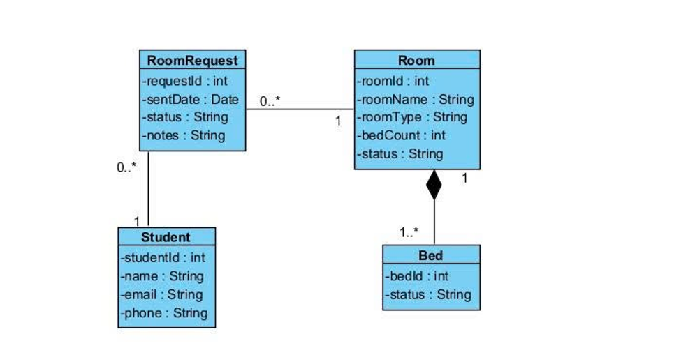
\includegraphics[width=0.72\textwidth]{assets/image4.png}
\caption{Sơ đồ lớp phân tích UC03 -- Sinh viên gửi yêu cầu đặt phòng}
\label{fig:uc03-class}
\end{figure}

\subsection{UC04 Cán bộ giữ phòng và giường cho sinh viên}

\subsubsection{Mục đích và mô tả chức năng}

\paragraph{Mục đích:}

Chức năng cho phép cán bộ xử lý yêu cầu đặt phòng của sinh viên bằng cách giữ một giường cụ thể cho sinh viên đó, hoặc từ chối yêu cầu khi không đáp ứng điều kiện. Dữ liệu giữ chỗ là đầu vào cho việc lập hợp đồng ở UC05.

\paragraph{Mô tả:}

Cán bộ xem danh sách yêu cầu đang chờ xử lý, chọn một yêu cầu và chọn giường cụ thể trong phòng phù hợp. Trước khi xác nhận, hệ thống kiểm tra lại trạng thái giường và xung đột thời gian để không giường nào bị giữ cho nhiều sinh viên. Khi thành công, hệ thống tạo bản ghi giữ chỗ, chuyển giường từ \textbf{trống} sang \textbf{đang giữ} và chuyển yêu cầu sang \textbf{Đã giữ chỗ}.

Để hạn chế hai yêu cầu đồng thời cùng giữ một giường, hệ thống có thể dùng khóa tạm có thời hạn trong Redis. Kết quả cuối cùng vẫn phải được kiểm tra và ghi nhận bằng giao dịch trong PostgreSQL.

\subsubsection{Tác nhân, tiền điều kiện và hậu điều kiện}

\begin{table}[H]
\centering
\small
\caption{Bảng dữ liệu đặc tả}
\label{tab:ch2-7}
\begin{tabularx}{\textwidth}{|>{\raggedright\arraybackslash}p{0.32\textwidth}|>{\raggedright\arraybackslash}X|}
\hline
\textbf{Mục} & \textbf{Nội dung} \\
\hline
\textbf{Use Case ID} & UC04 \\
\hline
\textbf{Tên Use Case} & Cán bộ giữ phòng và giường cho sinh viên \\
\hline
\textbf{Tác nhân chính} & Cán bộ quản lý ký túc xá \\
\hline
\textbf{Tác nhân phụ} & Không có tác nhân trực tiếp \\
\hline
\textbf{Tiền điều kiện} & Cán bộ đã đăng nhập và có quyền xử lý yêu cầu đặt phòng. Có ít nhất một yêu cầu ở trạng thái "Chờ xử lý". Phòng và giường liên quan đã tồn tại trong hệ thống. \\
\hline
\textbf{Hậu điều kiện thành công} & \textit{Trường hợp giữ chỗ:} một bản ghi giữ chỗ được tạo, gắn yêu cầu, sinh viên và giường; giường chuyển sang "đang giữ"; yêu cầu chuyển sang "Đã giữ chỗ". \textit{Trường hợp từ chối:} yêu cầu chuyển sang "Bị từ chối" kèm lý do; giường không thay đổi. \\
\hline
\textbf{Hậu điều kiện thất bại} & Không tạo bản ghi giữ chỗ; trạng thái giường và yêu cầu giữ nguyên như trước thao tác; khóa tạm (nếu đã tạo) được giải phóng. \\
\hline
\end{tabularx}
\end{table}

\subsubsection{Luồng sự kiện chính}

\begin{enumerate}[leftmargin=1.6em]
\item Cán bộ chọn chức năng \textbf{"Giữ phòng và giường"}.
\item Hệ thống hiển thị danh sách yêu cầu đặt phòng ở trạng thái "Chờ xử lý".
\item Cán bộ chọn một yêu cầu cần xử lý.
\item Hệ thống hiển thị thông tin yêu cầu (sinh viên, phòng đề nghị, ngày dự kiến bắt đầu, ghi chú) và danh sách giường đang trống của phòng.
\item Cán bộ chọn một giường cụ thể để giữ cho sinh viên.
\item Cán bộ chọn \textbf{"Xác nhận giữ chỗ"}.
\item Hệ thống kiểm tra lại tại thời điểm xử lý:
\begin{itemize}
\item Yêu cầu vẫn ở trạng thái "Chờ xử lý".
\item Giường vẫn ở trạng thái trống và chưa có khóa giữ hợp lệ.
\item Giường không xung đột thời gian với giữ chỗ hoặc hợp đồng khác.
\item Sinh viên không có hợp đồng lưu trú đang hiệu lực.
\end{itemize}
\item Hệ thống tạo khóa giữ giường có thời hạn cho giường được chọn.
\item Hệ thống mở giao dịch cơ sở dữ liệu và thực hiện đồng thời:
\begin{itemize}
\item Tạo bản ghi giữ chỗ (yêu cầu, sinh viên, giường, cán bộ, thời điểm giữ, thời hạn giữ).
\item Cập nhật trạng thái giường từ \textbf{trống} sang \textbf{đang giữ}.
\item Cập nhật trạng thái yêu cầu sang \textbf{Đã giữ chỗ}.
\end{itemize}
\item Hệ thống hoàn tất giao dịch và làm mới dữ liệu tìm phòng đã lưu tạm liên quan.
\item Hệ thống thông báo \textbf{"Giữ chỗ thành công"} cho cán bộ; sinh viên xem được kết quả xử lý yêu cầu của mình.
\end{enumerate}

\subsubsection{Luồng thay thế và ngoại lệ}

\paragraph{Luồng thay thế}

\begin{itemize}[leftmargin=1.4em]
\item 3a. Cán bộ từ chối yêu cầu:** Cán bộ chọn "Từ chối" và nhập lý do. Hệ thống chuyển yêu cầu sang "Bị từ chối", lưu lý do và không thay đổi dữ liệu giường. Sinh viên xem được kết quả và lý do.
\item 3b. Cán bộ không tiếp tục xử lý:** Cán bộ hủy thao tác. Hệ thống quay lại danh sách yêu cầu chờ xử lý và không thay đổi dữ liệu.
\item 4a. Phòng đề nghị không còn giường trống:** Hệ thống thông báo cho cán bộ. Cán bộ có thể chọn phòng khác còn chỗ phù hợp hoặc từ chối yêu cầu.
\item 7a. Yêu cầu không còn ở trạng thái chờ xử lý:** Hệ thống dừng thao tác, thông báo yêu cầu đã được xử lý và tải lại danh sách.
\item 7b. Giường đã bị giữ hoặc đang thuê:** Nếu giường đã có khóa giữ hợp lệ hoặc không còn trống (do cán bộ khác vừa xử lý), hệ thống từ chối và yêu cầu cán bộ chọn giường khác.
\item 7c. Sinh viên đã có hợp đồng đang hiệu lực:** Hệ thống không cho giữ chỗ và gợi ý cán bộ từ chối yêu cầu.
\item Luồng ngoại lệ**
\item 8a. Redis không khả dụng:** Hệ thống không xác nhận giữ chỗ chỉ dựa trên dữ liệu tạm. Hệ thống vẫn kiểm tra và khóa dữ liệu ngay trong giao dịch PostgreSQL rồi mới xác nhận (BR12).
\item 9a. Lỗi khi ghi dữ liệu:** Hệ thống hủy toàn bộ giao dịch, không tạo bản ghi giữ chỗ, giữ nguyên trạng thái giường và yêu cầu, giải phóng khóa tạm và thông báo lỗi cho cán bộ.
\item 9b. Xung đột đồng thời khi lưu:** Nếu giao dịch phát hiện giường vừa bị thay đổi bởi yêu cầu khác, hệ thống hủy giao dịch và thông báo cán bộ chọn lại giường.
\end{itemize}

\subsubsection{Quy tắc nghiệp vụ và dữ liệu liên quan}

\paragraph{Quy tắc nghiệp vụ}

\begin{itemize}[leftmargin=1.4em]
\item BR03:** Giường chỉ ở một trạng thái tại một thời điểm.
\item BR04:** Một giường không được giữ hoặc phân cho nhiều sinh viên cùng lúc.
\item BR12:** Trước khi giữ giường, hệ thống phải kiểm tra lại trạng thái tại thời điểm xử lý, không dùng dữ liệu cũ.
\item BR-UC04-01:** Chỉ giữ chỗ cho yêu cầu ở trạng thái "Chờ xử lý".
\item BR-UC04-02:** Chỉ giữ giường đang ở trạng thái trống; sau khi giữ, giường chuyển sang "đang giữ".
\item BR-UC04-03:** Một yêu cầu chỉ được giữ tối đa một giường; một sinh viên chỉ có một giữ chỗ hợp lệ tại một thời điểm.
\item BR-UC04-04:** Việc tạo giữ chỗ, cập nhật giường và cập nhật yêu cầu được thực hiện trong cùng một giao dịch: hoặc hoàn tất toàn bộ, hoặc không thay đổi gì.
\item BR-UC04-05:** Giữ chỗ có thời hạn. Nếu quá thời hạn mà chưa lập hợp đồng (UC05), giữ chỗ hết hiệu lực và giường quay về trạng thái trống.
\item BR-UC04-06:** Redis chỉ hỗ trợ khóa giữ tạm và tăng tốc; nếu Redis lỗi, tính đúng đắn vẫn dựa vào PostgreSQL.
\item BR-UC04-07:** Khi từ chối yêu cầu, cán bộ phải nhập lý do.
\item Dữ liệu liên quan**
\end{itemize}

\begin{table}[H]
\centering
\small
\caption{Bảng dữ liệu đặc tả}
\label{tab:ch2-8}
\begin{tabularx}{\textwidth}{|>{\raggedright\arraybackslash}p{0.28\textwidth}|>{\raggedright\arraybackslash}X|>{\raggedright\arraybackslash}p{0.28\textwidth}|}
\hline
\textbf{Đối tượng} & \textbf{Thuộc tính chính} & \textbf{Vai trò trong UC} \\
\hline
Yêu cầu đặt phòng (BookingRequest) & requestId, studentId, roomId, status, rejectReason & Được đọc và cập nhật trạng thái \\
\hline
Giữ chỗ (Reservation) & reservationId, requestId, studentId, bedId, staffId, reservedAt, expiresAt, status & Được tạo mới; là căn cứ lập hợp đồng ở UC05 \\
\hline
Giường (Bed) & bedId, roomId, status & Được kiểm tra và chuyển từ "trống" sang "đang giữ" \\
\hline
Phòng (Room) & roomId, building, roomType, fee & Cung cấp thông tin và danh sách giường \\
\hline
Sinh viên (Student) & studentId, họ tên & Người được giữ chỗ \\
\hline
Cán bộ (Staff) & staffId, họ tên & Người thực hiện giữ chỗ \\
\hline
Hợp đồng (Contract) & contractId, studentId, status & Chỉ đọc, dùng để kiểm tra BR06 \\
\hline
\end{tabularx}
\end{table}

\section{Phân tích nhóm chức năng thuê phòng}

\subsection{UC05 Cán bộ lập hợp đồng thuê phòng cho sinh viên}

\subsubsection{Mục đích và mô tả chức năng}

Mục đích:

Chức năng cho phép cán bộ quản lý ký túc xá lập hợp đồng thuê phòng cho sinh viên sau khi sinh viên đã được giữ một chỗ ở hợp lệ. Hợp đồng là cơ sở ghi nhận chính thức thông tin về sinh viên, phòng, giường, thời hạn lưu trú và mức phí áp dụng, đồng thời là đầu vào cho nghiệp vụ bàn giao phòng ở UC06.

Mô tả:

Sau khi sinh viên có một giường được giữ hợp lệ từ giai đoạn đặt phòng, cán bộ lựa chọn sinh viên cần lập hợp đồng. Hệ thống kiểm tra lại thông tin giữ chỗ, trạng thái hiện tại của giường và tình trạng hợp đồng của sinh viên. Nếu các điều kiện được đáp ứng, cán bộ nhập hoặc xác nhận các thông tin về thời hạn hợp đồng và mức phí. Hệ thống sau đó tạo và lưu hợp đồng.

Việc lập hợp đồng tại UC05 chưa đồng nghĩa sinh viên đã chính thức nhận phòng. Hợp đồng chỉ chuyển sang trạng thái có hiệu lực và giường chỉ chuyển sang trạng thái đang thuê sau khi cán bộ hoàn thành việc bàn giao phòng tại UC06

\subsubsection{Tác nhân, tiền điều kiện và hậu điều kiện}

\begin{table}[H]
\centering
\small
\caption{Bảng dữ liệu đặc tả}
\label{tab:ch2-9}
\begin{tabularx}{\textwidth}{|>{\raggedright\arraybackslash}p{0.32\textwidth}|>{\raggedright\arraybackslash}X|}
\hline
\textbf{Mục} & \textbf{Nội dung} \\
\hline
\textbf{Use Case ID} & UC05 \\
\hline
\textbf{Tên Use Case} & Cán bộ lập hợp đồng thuê phòng cho sinh viên \\
\hline
\textbf{Tác nhân chính} & Cán bộ quản lý ký túc xá \\
\hline
\textbf{Tác nhân phụ} & Không có tác nhân trực tiếp \\
\hline
\textbf{Tiền điều kiện} & Cán bộ đã đăng nhập và có quyền thực hiện chức năng lập hợp đồng. Sinh viên đã có một chỗ được giữ hợp lệ. Thông tin sinh viên, phòng và giường đã tồn tại trong hệ thống. \\
\hline
\textbf{Hậu điều kiện thành công} & Một hợp đồng lưu trú mới được tạo và lưu, gắn với sinh viên, phòng và giường đã được giữ. Hợp đồng ghi nhận thời gian bắt đầu, thời gian kết thúc, mức phí và trạng thái. Hợp đồng chưa chuyển sang trạng thái có hiệu lực cho đến khi bàn giao phòng thành công. \\
\hline
\textbf{Hậu điều kiện thất bại} & Không có hợp đồng mới được tạo; dữ liệu giữ chỗ, giường và các dữ liệu liên quan không bị thay đổi. \\
\hline
\end{tabularx}
\end{table}

\subsubsection{Luồng sự kiện chính}

\begin{enumerate}[leftmargin=1.6em]
\item Cán bộ chọn chức năng \textbf{“Lập hợp đồng thuê phòng”}.
\item Hệ thống hiển thị danh sách các sinh viên đã có chỗ được giữ hợp lệ và đủ điều kiện để lập hợp đồng.
\item Cán bộ lựa chọn sinh viên cần lập hợp đồng.
\item Hệ thống lấy thông tin giữ chỗ tương ứng và kiểm tra lại trạng thái hiện tại của sinh viên và giường.
\item Hệ thống kiểm tra:
\end{enumerate}

\begin{itemize}[leftmargin=1.4em]
\item Sinh viên có chỗ được giữ hợp lệ.
\item Giường vẫn đang được giữ cho đúng sinh viên.
\item Sinh viên không có hợp đồng lưu trú khác đang có hiệu lực.
\end{itemize}

\begin{enumerate}[leftmargin=1.6em]
\item Nếu các điều kiện được đáp ứng, hệ thống hiển thị thông tin lập hợp đồng gồm:
\end{enumerate}

\begin{itemize}[leftmargin=1.4em]
\item Thông tin sinh viên.
\item Thông tin phòng.
\item Thông tin giường.
\item Thời gian bắt đầu hợp đồng.
\item Thời gian kết thúc hợp đồng.
\item Mức phí áp dụng.
\end{itemize}

\begin{enumerate}[leftmargin=1.6em]
\item Cán bộ nhập hoặc xác nhận các thông tin của hợp đồng.
\item Cán bộ chọn \textbf{“Lập hợp đồng”}.
\item Hệ thống kiểm tra tính đầy đủ và hợp lệ của dữ liệu được nhập.
\item Hệ thống tạo bản ghi hợp đồng lưu trú, liên kết với sinh viên và chỗ ở đã được giữ.
\item Hệ thống lưu hợp đồng nhưng chưa chuyển hợp đồng sang trạng thái có hiệu lực.
\item Hệ thống thông báo \textbf{“Lập hợp đồng thành công”} cho cán bộ. Hợp đồng sau đó có thể được sử dụng trong UC06 – Cán bộ xác nhận bàn giao phòng cho sinh viên.
\end{enumerate}

\paragraph{d.Luồng thay thế}

\begin{itemize}[leftmargin=1.4em]
\item 3a. Cán bộ không tiếp tục lập hợp đồng:**
\end{itemize}

Cán bộ hủy thao tác. Hệ thống quay lại danh sách sinh viên/chỗ đã được giữ và không tạo hợp đồng.

\begin{itemize}[leftmargin=1.4em]
\item 4a. Thông tin giữ chỗ không còn hợp lệ:**
\end{itemize}

Hệ thống không cho phép tiếp tục lập hợp đồng và yêu cầu cán bộ kiểm tra lại thông tin giữ chỗ.

\begin{itemize}[leftmargin=1.4em]
\item 5a. Giường không còn ở trạng thái phù hợp:**
\end{itemize}

Nếu tại thời điểm kiểm tra, giường không còn được giữ hợp lệ cho sinh viên đang được chọn, hệ thống dừng quá trình lập hợp đồng và thông báo cho cán bộ.

\begin{itemize}[leftmargin=1.4em]
\item 5b. Sinh viên đã có hợp đồng đang có hiệu lực:**
\end{itemize}

Hệ thống từ chối lập hợp đồng mới và thông báo sinh viên đang có hợp đồng lưu trú còn hiệu lực.

\paragraph{e.Luồng ngoại lệ}

\begin{itemize}[leftmargin=1.4em]
\item 9a. Dữ liệu hợp đồng thiếu hoặc không hợp lệ:**
\end{itemize}

Hệ thống hiển thị thông tin lỗi tại trường tương ứng và yêu cầu cán bộ kiểm tra, chỉnh sửa trước khi tiếp tục.

\begin{itemize}[leftmargin=1.4em]
\item 10a. Có thay đổi trạng thái dữ liệu trong quá trình xử lý:**
\end{itemize}

Hệ thống kiểm tra lại trạng thái giường và dữ liệu giữ chỗ trước khi lưu. Nếu điều kiện không còn được đáp ứng, hợp đồng không được tạo.

\begin{itemize}[leftmargin=1.4em]
\item 11a. Lỗi khi lưu dữ liệu:**
\end{itemize}

Hệ thống không ghi nhận hợp đồng mới, giữ nguyên dữ liệu trước khi thực hiện thao tác và thông báo lỗi cho cán bộ.

Cách xử lý này phù hợp với yêu cầu chung của hệ thống là phải kiểm soát trạng thái để tránh việc một giường bị phân cho nhiều sinh viên

\subsubsection{Quy tắc nghiệp vụ và dữ liệu liên quan}
\textit{Phần này đang được bổ sung trong các phiên bản tiếp theo của báo cáo.}


\subsubsection{Sơ đồ lớp UC05}
\textit{Phần này đang được bổ sung trong các phiên bản tiếp theo của báo cáo.}


\subsection{UC06 Cán bộ xác nhận bàn giao phòng cho sinh viên}

\subsubsection{Mục đích và mô tả chức năng}

\paragraph{Mục đích:}

Chức năng cho phép cán bộ quản lý ký túc xá xác nhận việc bàn giao chỗ ở cho sinh viên sau khi hợp đồng thuê phòng đã được lập. Việc xác nhận bàn giao đánh dấu thời điểm sinh viên chính thức nhận và được quyền sử dụng giường đã được phân.

\paragraph{Mô tả:}

Sau khi UC05 hoàn tất việc lập hợp đồng, cán bộ lựa chọn hợp đồng cần thực hiện bàn giao. Hệ thống kiểm tra tính hợp lệ của hợp đồng và tình trạng hiện tại của giường. Nếu các điều kiện được đáp ứng, cán bộ xác nhận sinh viên đã nhận chỗ ở.

Khi bàn giao thành công, hệ thống ghi nhận thông tin bàn giao, chuyển hợp đồng sang trạng thái \textbf{có hiệu lực} và cập nhật trạng thái giường từ \textbf{đang giữ} sang \textbf{đang thuê}.

\subsubsection{Tác nhân, tiền điều kiện và hậu điều kiện}

\begin{table}[H]
\centering
\small
\caption{Bảng dữ liệu đặc tả}
\label{tab:ch2-10}
\begin{tabularx}{\textwidth}{|>{\raggedright\arraybackslash}p{0.32\textwidth}|>{\raggedright\arraybackslash}X|}
\hline
\textbf{Mục} & \textbf{Nội dung} \\
\hline
\textbf{Use Case ID} & UC06 \\
\hline
\textbf{Tên Use Case} & Cán bộ xác nhận bàn giao phòng cho sinh viên \\
\hline
\textbf{Tác nhân chính} & Cán bộ quản lý ký túc xá \\
\hline
\textbf{Tác nhân phụ} & Không có tác nhân trực tiếp \\
\hline
\textbf{Tiền điều kiện} & Cán bộ đã đăng nhập và có quyền thực hiện chức năng bàn giao. Sinh viên đã có hợp đồng thuê phòng được lập hợp lệ. Giường liên kết với hợp đồng vẫn đang được giữ cho sinh viên và chưa được phân cho người khác. \\
\hline
\textbf{Hậu điều kiện thành công} & Thông tin bàn giao được ghi nhận; hợp đồng chuyển sang trạng thái có hiệu lực; giường chuyển từ trạng thái đang giữ sang đang thuê. \\
\hline
\textbf{Hậu điều kiện thất bại} & Không ghi nhận bàn giao; hợp đồng và trạng thái giường giữ nguyên trạng thái trước khi thực hiện thao tác. \\
\hline
\end{tabularx}
\end{table}

\subsubsection{Luồng sự kiện chính}

Cán bộ chọn chức năng \textbf{“Xác nhận bàn giao phòng”}.

Hệ thống hiển thị các hợp đồng đã được lập và đang chờ thực hiện bàn giao.

Cán bộ lựa chọn hợp đồng của sinh viên cần bàn giao phòng.

Hệ thống hiển thị các thông tin liên quan gồm:

\begin{itemize}[leftmargin=1.4em]
\item Thông tin sinh viên.
\item Thông tin hợp đồng.
\item Phòng được phân.
\item Giường được phân.
\item Thời gian của hợp đồng.
\item Mức phí áp dụng.
\item Trạng thái hiện tại của hợp đồng và giường.
\end{itemize}

Hệ thống kiểm tra điều kiện bàn giao:

\begin{itemize}[leftmargin=1.4em]
\item Hợp đồng tồn tại và hợp lệ.
\item Hợp đồng chưa được bàn giao trước đó.
\item Giường vẫn đang được giữ cho đúng sinh viên.
\item Sinh viên không có hợp đồng lưu trú khác đang có hiệu lực.
\item Giường chưa được phân cho sinh viên khác.
\end{itemize}

Khi các điều kiện được đáp ứng, hệ thống cho phép cán bộ thực hiện xác nhận bàn giao.

Cán bộ chọn \textbf{“Xác nhận bàn giao”}.

Hệ thống ghi nhận thông tin bàn giao phòng.

Hệ thống cập nhật trạng thái hợp đồng sang \textbf{có hiệu lực}.

Hệ thống cập nhật trạng thái giường từ \textbf{đang giữ} sang \textbf{đang thuê}.

Hệ thống lưu toàn bộ thay đổi.

Hệ thống thông báo \textbf{“Bàn giao phòng thành công”} cho cán bộ.

\subsubsection{Luồng thay thế}

\paragraph{3a. Cán bộ không tiếp tục bàn giao}

Cán bộ hủy thao tác. Hệ thống quay trở lại danh sách hợp đồng chờ bàn giao và không thay đổi dữ liệu.

\paragraph{5a. Hợp đồng không còn hợp lệ}

Nếu hợp đồng không tồn tại hoặc không còn ở trạng thái phù hợp để bàn giao, hệ thống từ chối thao tác và thông báo cho cán bộ kiểm tra lại hợp đồng.

\paragraph{5b. Hợp đồng đã được bàn giao trước đó}

Nếu hợp đồng đã có hiệu lực do quá trình bàn giao đã được thực hiện, hệ thống không cho phép xác nhận bàn giao lần nữa.

\paragraph{5c. Giường không còn được giữ cho sinh viên}

Nếu tại thời điểm xử lý, trạng thái giường không còn phù hợp hoặc giường không còn gắn với đúng sinh viên trong hợp đồng, hệ thống dừng quá trình bàn giao và thông báo cho cán bộ.

\paragraph{5d. Sinh viên đã có hợp đồng khác đang có hiệu lực}

Hệ thống không cho phép bàn giao hợp đồng mới để tránh một sinh viên đồng thời có nhiều hợp đồng lưu trú còn hiệu lực.

\subsubsection{Luồng ngoại lệ}

\paragraph{8a. Không thể ghi nhận thông tin bàn giao}

Nếu xảy ra lỗi khi tạo dữ liệu bàn giao, hệ thống không thực hiện cập nhật trạng thái hợp đồng và giường.

\paragraph{9a. Cập nhật hợp đồng thất bại}

Nếu không thể chuyển hợp đồng sang trạng thái có hiệu lực, toàn bộ thao tác bàn giao bị hủy.

\paragraph{10a. Cập nhật trạng thái giường thất bại}

Nếu hợp đồng đã được xử lý nhưng không thể cập nhật giường sang trạng thái đang thuê, hệ thống phải hủy toàn bộ thay đổi để không tạo ra trạng thái dữ liệu không nhất quán.

\subsubsection{Quy tắc nghiệp vụ và dữ liệu liên quan}
\textit{Phần này đang được bổ sung trong các phiên bản tiếp theo của báo cáo.}


\subsubsection{Sơ đồ lớp UC06}
\textit{Phần này đang được bổ sung trong các phiên bản tiếp theo của báo cáo.}


\section{Phân tích nhóm chức năng đóng phí}

\subsection{UC07 Hệ thống lập khoản phí nội trú cho sinh viên}

\subsubsection{Mục đích và mô tả chức năng}

Mục đích: tự động lập các khoản phí nội trú theo từng kỳ cho sinh viên đang ở KTX, để sinh viên có căn cứ thanh toán (UC08).

Mô tả: đến kỳ thu phí, cán bộ kích hoạt chức năng. Hệ thống lấy các hợp đồng còn hiệu lực, tính số tiền theo phí phòng, tạo bản ghi DormitoryFee với trạng thái "Chưa thanh toán" và thông báo cho sinh viên.

\subsubsection{Tác nhân, tiền điều kiện và hậu điều kiện}

Tác nhân chính : Cán bộ quản lý ký túc xá

Tác nhân phụ: Không có

Tiền điều kiện: Cán bộ đã đăng nhập vào hệ thống và có quyền quản lý tài chính/khoản phí. Dữ liệu danh mục kỳ thu, loại phí đã được thiết lập. Tồn tại ít nhất một hợp đồng thuê phòng đang có hiệu lực (ACTIVE) trong kỳ thu tương ứng.

Hậu điều kiện thành công: Các bản ghi khoản phí nội trú mới được tạo và lưu vào cơ sở dữ liệu với trạng thái "Chưa thanh toán". Sinh viên có thể tra cứu thấy khoản nợ phát sinh của mình trên hệ thống.

Hậu điều kiện thất bại: Không có khoản phí nào được tạo hoặc dữ liệu bị hủy toàn bộ nếu có lỗi giao dịch; thông tin công nợ giữ nguyên trạng thái trước đó.

\subsubsection{Luồng sự kiện chính}

Cán bộ chọn chức năng "Phát hành khoản phí nội trú theo kỳ".

Hệ thống hiển thị biểu mẫu chọn kỳ thu, loại phí và hạn nộp tiền.

Cán bộ chọn kỳ thu cần tính phí, nhập hạn nộp và chọn "Kiểm tra danh sách hợp đồng".

Hệ thống quét cơ sở dữ liệu, lọc các hợp đồng đang có hiệu lực (ACTIVE) và kiểm tra điều kiện phát sinh phí (chưa được lập phí cho kỳ này).

Hệ thống hiển thị danh sách dự kiến các khoản phí (Mã SV, họ tên, mã hợp đồng, phòng, số tiền theo tháng/kỳ, hạn nộp) để cán bộ đối chiếu.

Cán bộ kiểm tra danh sách và chọn "Xác nhận phát hành phí".

Hệ thống mở giao dịch cơ sở dữ liệu (PostgreSQL Transaction):

\begin{itemize}[leftmargin=1.4em]
\item Tạo các bản ghi Fee tương ứng với từng hợp đồng.
\item Thiết lập trạng thái khoản phí là UNPAID ("Chưa thanh toán").
\item Ghi nhận ngày tạo, hạn thanh toán và cán bộ thực hiện.
\end{itemize}

Hệ thống hoàn tất giao dịch cơ sở dữ liệu.

Hệ thống gửi thông báo khoản phí mới vào trang quản lý của các sinh viên liên quan.

Hệ thống hiển thị thông báo "Phát hành khoản phí nội trú thành công" kèm tổng số lượng bản ghi đã tạo.

\subsubsection{Luồng thay thế và ngoại lệ}

\paragraph{Luồng thay thế:}

\begin{itemize}[leftmargin=1.4em]
\item 3a. Cán bộ hủy thao tác: Cán bộ chọn hủy; hệ thống quay trở lại màn hình quản trị tài chính, không lưu dữ liệu.
\item 4a. Không tìm thấy hợp đồng đủ điều kiện: Hệ thống thông báo không có hợp đồng đang hiệu lực hoặc các hợp đồng đã được tạo phí cho kỳ này, dừng quá trình phát hành.
\item 6a. Cán bộ điều chỉnh danh sách: Cán bộ có thể bỏ chọn một số sinh viên có trường hợp đặc biệt (ví dụ miễn giảm) trước khi phát hành hàng loạt.
\item Luồng ngoại lệ:**
\item 2a. Hạn thanh toán không hợp lệ: Nếu cán bộ nhập hạn thanh toán nhỏ hơn hoặc bằng ngày phát hành, hệ thống báo lỗi và yêu cầu chọn lại.
\item 7a. Lỗi ghi dữ liệu/xung đột giao dịch: Hệ thống rollback toàn bộ giao dịch, không tạo khoản phí dở dang và báo lỗi cho cán bộ.
\end{itemize}

\subsubsection{Quy tắc nghiệp vụ và dữ liệu liên quan}

Quy tắc nghiệp vụ:

\begin{itemize}[leftmargin=1.4em]
\item BR01, BR02: Chỉ cán bộ quản lý mới có quyền phát hành khoản phí.
\item BR08: Chỉ phát sinh và phát hành khoản phí cho các hợp đồng đang có hiệu lực (status = ACTIVE).
\item BR-UC07-01: Mỗi hợp đồng chỉ được phát hành một khoản phí nội trú duy nhất cho mỗi kỳ.
\item BR-UC07-02: Hạn nộp phí phải sau thời điểm phát hành.
\item BR-UC07-03: Toàn bộ các bản ghi phí trong đợt phát hành phải được tạo trong cùng một giao dịch toàn vẹn (ACID).
\end{itemize}

Dữ liệu liên quan:

\subsubsection{Sơ đồ lớp UC07}
\textit{Phần này đang được bổ sung trong các phiên bản tiếp theo của báo cáo.}


\subsection{UC08 Sinh viên thanh toán khoản phí nội trú}

\subsubsection{a Mục đích và mô tả chức năng}

Mục đích: Cho phép sinh viên tra cứu công nợ cá nhân và thực hiện thanh toán các khoản phí nội trú đang ở trạng thái chưa thanh toán.

Mô tả: Sinh viên đăng nhập vào hệ thống, xem danh sách các khoản phí nội trú của mình, chọn khoản phí cần thanh toán và chọn phương thức thanh toán. Hệ thống kiểm tra tính hợp lệ của khoản phí, mô phỏng/ghi nhận kết quả giao dịch thanh toán (Payment Transaction), cập nhật trạng thái khoản phí sang "Đã thanh toán" và lưu biên lai giao dịch.

\subsubsection{Tác nhân, tiền điều kiện và hậu điều kiện}

Tác nhân chính: Sinh viên

Tác nhân phụ: Cổng thanh toán / Hệ thống mô phỏng thanh toán

Tiền điều kiện: Sinh viên đã đăng nhập hệ thống. Tồn tại ít nhất một khoản phí của sinh viên có trạng thái "Chưa thanh toán" (status = UNPAID).

Hậu điều kiện thành công: Giao dịch thanh toán (PaymentTransaction) được tạo và lưu trữ. Khoản phí chuyển sang trạng thái "Đã thanh toán" (PAID). Sinh viên nhận được biên lai giao dịch thành công.

Hậu điều kiện thất bại: Giao dịch thất bại; trạng thái khoản phí vẫn là UNPAID; không ghi nhận biến động công nợ.

\subsubsection{Luồng sự kiện chính}

Sinh viên chọn chức năng "Khoản phí nội trú".

Hệ thống truy vấn và hiển thị danh sách các khoản phí của sinh viên (kỳ thu, số tiền, hạn nộp, trạng thái).

Sinh viên chọn một khoản phí đang ở trạng thái UNPAID và bấm "Thanh toán".

Hệ thống kiểm tra lại trạng thái khoản phí tại thời điểm thanh toán (đảm bảo vẫn là UNPAID và chưa bị khóa bởi giao dịch đang xử lý).

Hệ thống hiển thị màn hình xác nhận thanh toán (Mã khoản phí, tên sinh viên, số tiền cần đóng, phương thức thanh toán).

Sinh viên chọn phương thức thanh toán (ví dụ: chuyển khoản/mô phỏng cổng thanh toán) và chọn "Xác nhận thanh toán".

Hệ thống chuyển tiếp yêu cầu đến module xử lý/mô phỏng thanh toán.

Hệ thống nhận phản hồi thanh toán thành công.

Hệ thống mở giao dịch cơ sở dữ liệu:

\begin{itemize}[leftmargin=1.4em]
\item Tạo bản ghi giao dịch PaymentTransaction với mã giao dịch, số tiền, phương thức, thời gian thanh toán và kết quả SUCCESS.
\item Cập nhật trạng thái của bản ghi Fee từ UNPAID sang PAID.
\end{itemize}

Hệ thống lưu thành công giao dịch vào PostgreSQL.

Hệ thống hiển thị thông báo "Thanh toán thành công" và xuất biên lai thanh toán cho sinh viên.

\subsubsection{Luồng thay thế và ngoại lệ}

Luồng thay thế:

\begin{itemize}[leftmargin=1.4em]
\item 3a. Sinh viên hủy giao dịch: Sinh viên nhấn hủy tại bước xác nhận; hệ thống quay lại màn hình danh sách khoản phí, không thay đổi dữ liệu.
\item 4a. Khoản phí đã được thanh toán: Nếu khoản phí vừa được gạch nợ ở phiên khác, hệ thống thông báo "Khoản phí này đã được thanh toán" và tải lại danh sách.
\end{itemize}

Luồng ngoại lệ:

\begin{itemize}[leftmargin=1.4em]
\item 7a. Quá trình xử lý thanh toán bị từ chối / không thành công: Cổng thanh toán mô phỏng phản hồi giao dịch thất bại; hệ thống tạo bản ghi PaymentTransaction với trạng thái FAILED, giữ nguyên trạng thái UNPAID của khoản phí và hiển thị thông báo nguyên nhân thất bại cho sinh viên.
\item 9a. Lỗi cơ sở dữ liệu khi cập nhật: Hệ thống hủy giao dịch (rollback), trạng thái khoản phí không thay đổi và hiển thị cảnh báo để sinh viên đối soát.
\end{itemize}

\subsubsection{Quy tắc nghiệp vụ và dữ liệu liên quan}
\textit{Phần này đang được bổ sung trong các phiên bản tiếp theo của báo cáo.}


\subsubsection{Sơ đồ lớp UC08}
\textit{Phần này đang được bổ sung trong các phiên bản tiếp theo của báo cáo.}


\section{Phân tích nhóm chức năng trả phòng}

\subsection{UC09 Sinh viên gửi yêu cầu trả phòng}

\subsubsection{Mục đích và mô tả chức năng}

Mục đích:

Chức năng cho phép sinh viên đang lưu trú tại ký túc xá gửi yêu cầu trả phòng khi không còn nhu cầu tiếp tục sử dụng chỗ ở. Yêu cầu được ghi nhận trên hệ thống và là cơ sở để cán bộ quản lý thực hiện xác nhận hoàn tất trả phòng tại UC10

Mô tả:

Sinh viên đăng nhập vào hệ thống và lựa chọn chức năng gửi yêu cầu trả phòng. Hệ thống kiểm tra hợp đồng lưu trú đang có hiệu lực và hiển thị thông tin phòng, giường tương ứng.

Sinh viên nhập thời gian dự kiến trả phòng và các thông tin cần thiết, sau đó xác nhận gửi yêu cầu. Hệ thống kiểm tra tính hợp lệ của dữ liệu và lưu yêu cầu với trạng thái "Chờ xử lý".

Sau khi gửi thành công, sinh viên có thể theo dõi trạng thái yêu cầu. Việc gửi yêu cầu chưa làm thay đổi trạng thái hợp đồng hoặc giải phóng giường.

\subsubsection{Tác nhân, tiền điều kiện và hậu điều kiện}

\begin{table}[H]
\centering
\small
\caption{Bảng dữ liệu đặc tả}
\label{tab:ch2-11}
\begin{tabularx}{\textwidth}{|>{\raggedright\arraybackslash}p{0.32\textwidth}|>{\raggedright\arraybackslash}X|}
\hline
\textbf{Mục} & \textbf{Nội dung} \\
\hline
\textbf{Use Case ID} & UC09 \\
\hline
\textbf{Tên Use Case} & Sinh viên gửi yêu cầu trả phòng \\
\hline
\textbf{Tác nhân chính} & Sinh viên \\
\hline
\textbf{Tác nhân phụ} & Không có \\
\hline
\textbf{Tiền điều kiện} & Sinh viên đã đăng nhập vào hệ thống và có hợp đồng lưu trú đang có hiệu lực. Thông tin phòng và giường tương ứng đã tồn tại trong hệ thống. \\
\hline
\textbf{Hậu điều kiện thành công} & Yêu cầu trả phòng được tạo và lưu với trạng thái "Chờ xử lý". Hệ thống ghi nhận thông tin sinh viên, hợp đồng và thời gian dự kiến trả phòng. \\
\hline
\textbf{Hậu điều kiện thất bại} & Không có yêu cầu trả phòng mới được tạo. Thông tin hợp đồng và trạng thái giường không thay đổi. \\
\hline
\end{tabularx}
\end{table}

\subsubsection{Luồng sự kiện chính}

Luồng sự kiện chính của UC09 được thực hiện như sau:

\begin{enumerate}[leftmargin=1.6em]
\item Sinh viên đăng nhập vào hệ thống và lựa chọn chức năng "Gửi yêu cầu trả phòng".
\item Hệ thống tìm kiếm và kiểm tra hợp đồng lưu trú đang có hiệu lực của sinh viên.
\item Hệ thống hiển thị thông tin hợp đồng, phòng và giường mà sinh viên đang sử dụng.
\item Sinh viên nhập thời gian dự kiến trả phòng và ghi chú nếu có.
\item Sinh viên kiểm tra thông tin và nhấn nút "Gửi yêu cầu".
\item Hệ thống kiểm tra tính đầy đủ, hợp lệ của thông tin và trạng thái hợp đồng tại thời điểm xử lý.
\item Nếu dữ liệu hợp lệ, hệ thống tạo bản ghi yêu cầu trả phòng, liên kết với sinh viên và hợp đồng tương ứng.
\item Hệ thống thiết lập trạng thái yêu cầu là "Chờ xử lý" và ghi nhận thời điểm gửi.
\item Hệ thống lưu thông tin yêu cầu trả phòng vào cơ sở dữ liệu.
\item Hệ thống hiển thị thông báo gửi yêu cầu thành công. Sinh viên có thể theo dõi trạng thái xử lý của yêu cầu.
\end{enumerate}

\subsubsection{Luồng thay thế và ngoại lệ}

\paragraph{Luồng thay thế:}

\begin{itemize}[leftmargin=1.4em]
\item 2a. Sinh viên không có hợp đồng đang hiệu lực:** Hệ thống thông báo sinh viên không có hợp đồng hợp lệ và không cho phép gửi yêu cầu trả phòng.
\item 4a. Sinh viên không nhập ghi chú:** Hệ thống cho phép tiếp tục thực hiện vì ghi chú là thông tin không bắt buộc.
\item 5a. Sinh viên hủy thao tác:** Hệ thống quay lại màn hình quản lý hợp đồng và không tạo yêu cầu trả phòng.
\item Luồng ngoại lệ:**
\item 1a. Phiên đăng nhập không hợp lệ:** Hệ thống yêu cầu sinh viên đăng nhập lại trước khi tiếp tục thao tác.
\item 6a. Thông tin không hợp lệ:** Hệ thống hiển thị thông báo lỗi và yêu cầu sinh viên chỉnh sửa thông tin.
\item 6b. Trạng thái hợp đồng thay đổi:** Nếu hợp đồng không còn hiệu lực tại thời điểm xử lý, hệ thống từ chối tạo yêu cầu.
\item 9a. Lỗi lưu dữ liệu:** Hệ thống thông báo lỗi, không tạo yêu cầu trả phòng và giữ nguyên dữ liệu hiện tại.
\end{itemize}

\subsubsection{Quy tắc nghiệp vụ và dữ liệu liên quan}
\textit{Phần này đang được bổ sung trong các phiên bản tiếp theo của báo cáo.}


\subsubsection{Biểu đồ hoạt động UC09}
\textit{Phần này đang được bổ sung trong các phiên bản tiếp theo của báo cáo.}


\subsection{UC10 Cán bộ xác nhận hoàn tất trả phòng}

\subsubsection{Mục đích và mô tả chức năng}
\textit{Phần này đang được bổ sung trong các phiên bản tiếp theo của báo cáo.}


\subsubsection{Tác nhân, tiền điều kiện và hậu điều kiện}
\textit{Phần này đang được bổ sung trong các phiên bản tiếp theo của báo cáo.}


\subsubsection{Luồng sự kiện chính}
\textit{Phần này đang được bổ sung trong các phiên bản tiếp theo của báo cáo.}


\subsubsection{Luồng thay thế và ngoại lệ}
\textit{Phần này đang được bổ sung trong các phiên bản tiếp theo của báo cáo.}


\subsubsection{Quy tắc nghiệp vụ và dữ liệu liên quan}
\textit{Phần này đang được bổ sung trong các phiên bản tiếp theo của báo cáo.}


\subsubsection{Biểu đồ hoạt động UC10}

\#\#\#

\#\#

\clearpage
\chapter*{KẾT LUẬN VÀ HƯỚNG PHÁT TRIỂN}
\phantomsection
\addcontentsline{toc}{chapter}{KẾT LUẬN VÀ HƯỚNG PHÁT TRIỂN}

\section*{Kết luận}
\phantomsection
\addcontentsline{toc}{section}{Kết luận}

Báo cáo đã xác định bài toán quản lý vòng đời chỗ ở tại ký túc xá PTIT và giới hạn phạm vi thành mười chức năng, chia theo năm giai đoạn: xem phòng, đặt phòng, thuê phòng, đóng phí và trả phòng. Các quy tắc nghiệp vụ then chốt đã được hệ thống hóa (BR01--BR12), bảo đảm một giường không bị giữ trùng, một sinh viên không có hai hợp đồng còn hiệu lực và các thay đổi trạng thái được thực hiện đồng bộ.

Phần phân tích đã xây dựng danh sách Use Case, ma trận tác nhân -- Use Case và đặc tả chi tiết các chức năng UC03, UC04, UC05, UC06, UC07, UC08, UC09. Định hướng công nghệ được lựa chọn gồm ReactJS cho giao diện, Java cho backend, PostgreSQL cho dữ liệu chính và Redis cho hỗ trợ tra cứu, giữ chỗ tạm.

\section*{Hướng phát triển}
\phantomsection
\addcontentsline{toc}{section}{Hướng phát triển}

Trong các giai đoạn tiếp theo, nhóm sẽ hoàn thiện các mục còn thiếu ở Chương 2 (đặc tả UC01, UC02, UC10 và các sơ đồ lớp, biểu đồ Use Case), sau đó chuyển sang thiết kế kiến trúc, cơ sở dữ liệu, giao diện và cài đặt minh họa luồng dữ liệu từ tạo phòng đến hoàn tất trả phòng.

Các hướng mở rộng gồm tích hợp cổng thanh toán thực tế, thông báo tự động, quản lý điện nước, tài sản, sửa chữa cơ sở vật chất, vi phạm nội trú và đồng bộ với hệ thống đào tạo, trên cơ sở vẫn giữ nguyên các ràng buộc toàn vẹn dữ liệu đã phân tích.

\clearpage
\chapter*{TÀI LIỆU THAM KHẢO}
\phantomsection
\addcontentsline{toc}{chapter}{TÀI LIỆU THAM KHẢO}

\begin{enumerate}[leftmargin=1.8em]
\item Nguyễn Văn Vy, Nguyễn Văn Hòa, \textit{Phân tích thiết kế hệ thống thông tin}, NXB Giáo dục Việt Nam.
\item Nguyễn Văn Ba, \textit{Phân tích và thiết kế hệ thống thông tin}, NXB Đại học Quốc gia Hà Nội.
\item Booch, G., Rumbaugh, J., Jacobson, I., \textit{The Unified Modeling Language User Guide}, Addison-Wesley.
\item React, \textit{React documentation}, \url{https://react.dev/}.
\item Oracle, \textit{Java documentation}, \url{https://docs.oracle.com/en/java/}.
\item PostgreSQL Global Development Group, \textit{PostgreSQL documentation}, \url{https://www.postgresql.org/docs/}.
\item Redis Ltd., \textit{Redis documentation}, \url{https://redis.io/docs/}.
\end{enumerate}

\clearpage
\chapter*{PHỤ LỤC}
\phantomsection
\addcontentsline{toc}{chapter}{PHỤ LỤC}

\section*{PHỤ LỤC A. Danh sách Use Case}
\phantomsection
\addcontentsline{toc}{section}{PHỤ LỤC A. Danh sách Use Case}

Mười chức năng trong phạm vi đề tài: UC01 Tạo phòng và giường; UC02 Tìm phòng còn chỗ phù hợp; UC03 Gửi yêu cầu đặt phòng; UC04 Giữ phòng và giường; UC05 Lập hợp đồng thuê phòng; UC06 Xác nhận bàn giao phòng; UC07 Phát hành khoản phí nội trú theo kỳ; UC08 Thanh toán khoản phí nội trú; UC09 Gửi yêu cầu trả phòng; UC10 Xác nhận hoàn tất trả phòng.

\section*{PHỤ LỤC B. Quy tắc nghiệp vụ chung}
\phantomsection
\addcontentsline{toc}{section}{PHỤ LỤC B. Quy tắc nghiệp vụ chung}

Các quy tắc BR01--BR12 được trình bày tại Mục 2.1.6, Chương 2.

\section*{PHỤ LỤC C. Các sơ đồ UML}
\phantomsection
\addcontentsline{toc}{section}{PHỤ LỤC C. Các sơ đồ UML}

Các sơ đồ Use Case tổng quát, sơ đồ lớp và biểu đồ hoạt động sẽ được tập hợp tại phụ lục này khi hoàn thiện mô hình.

\clearpage
\chapter*{BẢNG PHÂN CÔNG CÔNG VIỆC CÁC THÀNH VIÊN}
\phantomsection
\addcontentsline{toc}{chapter}{BẢNG PHÂN CÔNG CÔNG VIỆC CÁC THÀNH VIÊN}

Theo phân công trong danh sách Use Case:

\begin{table}[H]
\centering
\begin{tabularx}{\textwidth}{|>{\raggedright\arraybackslash}p{0.14\textwidth}|>{\raggedright\arraybackslash}X|>{\raggedright\arraybackslash}p{0.22\textwidth}|>{\raggedright\arraybackslash}p{0.18\textwidth}|}
\hline
\textbf{Mã} & \textbf{Use Case} & \textbf{Tác nhân} & \textbf{Phụ trách} \\
\hline
UC01 & Tạo phòng và giường & Cán bộ & Tùng \\
\hline
UC02 & Tìm phòng còn chỗ phù hợp & Sinh viên & Tùng \\
\hline
UC03 & Gửi yêu cầu đặt phòng & Sinh viên & Nhân \\
\hline
UC04 & Giữ phòng và giường cho sinh viên & Cán bộ & Nhân \\
\hline
UC05 & Lập hợp đồng thuê phòng cho sinh viên & Cán bộ & Huân \\
\hline
UC06 & Xác nhận bàn giao phòng cho sinh viên & Cán bộ & Huân \\
\hline
UC07 & Phát hành khoản phí nội trú theo kỳ & Cán bộ & Tuấn \\
\hline
UC08 & Thanh toán khoản phí nội trú & Sinh viên & Tuấn \\
\hline
UC09 & Gửi yêu cầu trả phòng & Sinh viên & Dũng \\
\hline
UC10 & Xác nhận hoàn tất trả phòng & Cán bộ & Dũng \\
\hline
\end{tabularx}
\caption{Phân công phụ trách các Use Case}
\label{tab:work-assignment}
\end{table}


\end{document}
